\chapter{Supporting material for ``Associations between the gut microbiome and metabolime in early life"}

\section{Supplemental Notes} 
\subsection{Supplementary Note 1} \label{appB_note1}
{\bf Microbe-metabolite participation in significant pairwise Spearman correlation}. Univariate pairwise Spearman correlations were performed to identify significant microbe-metabolite pairs. Significance was determined by the Spearman false discovery rate (FDR) threshold of 0.05 following a Benjamini-Hochberg multiple hypothesis testing procedure.  At both time points a majority of genera and metabolites were significantly correlated, where at 6 weeks, 28 genera (65\% of total genera) and 36 metabolites (100\% of metabolites) were part of 516 significant correlations (16.6\% of total pairwise comparisons) while at 12 months, 59 genera (81.9\% of total genera) and 29 metabolites (80\% of metabolites) were involved in 214 significant correlations (8.01\% of total pairwise comparisons). This result also supported the observation that at 6 weeks the microbiome was marginally more associated with the metabolome compared to 12 months. Similar to sCCA results, untargeted data set showed a similar signal at both time points. Specifically, at 6 weeks, 37 genera (86\% of genera) and 198 metabolite bins (95.1\% of bins) were part of 1480 significant associations (16.5\% of pairwise comparisons). Similarly, at 12 months, 67 genera (93\% of genera) and 207 metabolite bins (99.5\% of bins) were part of 1392 significant associations (9.2\% of total pairwise comparisons). 

\subsection{Supplementary Note 2} \label{appB_note2}
{\bf Sparse canonical correlation analysis selects microbes and metabolites important to the inter-omic correlation.} Only a small subset of metabolites and microbes were selected (27\% of taxa for both time points; 16.9\% of metabolites at 6 weeks and 19.4\% of metabolites at 12 months). At both time points, selected taxa belong to the Firmicutes, Actinobacteria and Proteobacteria phyla with Firmicutes being the most represented (58.3\% of selected taxa at 6 weeks; 70\% of selected taxa at 12 months). Actinobacteria was the second most selected phylum (25\% of selected taxa) at 6 weeks while at 12 months it was Proteobacteria (30\% of selected taxa). For metabolites, amino acids were the most represented metabolite class (\nameref{appB_note4}) (60\% of selected metabolites at 6 weeks, 85\% of selected metabolites at 12 months). 6-week samples demonstrated a larger diversity of metabolite classes, with additional representatives from carboxylic acids group, nucleotides and short chain fatty acids (SCFA) while at 12 months, the only non-amino-acid metabolite is uracil (of the nucleotide class). Across both time points, 3 genera (Flavonifractor, Haemophilus and Acinetobacter genera) and 5 metabolites (lysine, isoleucine, leucine, uracil, phenylalanine) were consistently selected. Surprisingly, in the untargeted analysis, nearly half of taxa and metabolites were selected at 6 weeks while the number remained more similar to the targeted analysis at 12 months (6 weeks: 46\% of taxa and 42\% of metabolite bins; 12 months: 13.8\% of taxa and  17.3\% of metabolite bins). However, the taxonomic distribution of those selected taxa remained similar, with Firmicutes being the most dominating phyla (60\% of selected taxa at both time points). Additionally, for both time points, the sign of the sCCA loadings for selected variables were also concordant with patterns of negative and positive correlation via univariate Spearman correlations (Figure 3, right panels). Notably, all selected metabolites contain negative loadings for both time points, with the majority of selected pairwise correlation to be negative (6 weeks: 76.6\% of selected pairwise comparisons, 12 months: 60.7\% of selected pairwise comparisons). This pattern is replicated in the untargeted data set as well (6 weeks: 61.3\% of selected pairwise comparisons, 12 months: 70\% of selected pairwise comparisons). 

\subsection{Supplementary Note 3} \label{appB_note3}
\textbf{Prediction results.} Under $R^2$, at 6 weeks only 8 (22.2\%) metabolites (Butyrate, Glycerol, Isobutyrate, Isoleucine, Leucine, Methionine, Phenylalanine and Tyrosine) were predictable, with a mean of 4.85\% and a maximum of 11.8\% (Butyrate using EN). At 12 months, only 14 (38.9\%) of metabolites (Butyrate, Formate, Inosine, Isobutyerate, Isoleucine, Lactate, Leucine, Methionine, Phenylalanine, Propionate, Propylene glycol, Tyrosine, Uracil, Valine) were predictable, with a mean of 4.81\% and a maximum of 8.7\% (Propylene Glycol using RF). When looking at the average R2 across all metabolites, performance was not good (-5.6\% at 6 weeks; -3.07\% at 12 months). This negative $R_2$ value implies that the predicted model performs worse than the naïve, intercept only model. Conversely, correlative performance was much better. At 6 weeks 26 metabolites (83\%) were predictable, with a mean correlation of 0.344 and a maximum of 0.669 (Butyrate using EN). Similarly, at 12 months all 36 targeted metabolites were predictable, with a mean of 0.265 and a maximum of 0.549 (Succinate using EN). Using the SCC cutoff of 0.3 as criteria for well predicted metabolites, many metabolites at 6 weeks were still retained (25 metabolites - 69.4\%). Conversely, at 12 months, only 13 metabolites remained to be well predicted (38.9\%). On average, performance based on SCC was good with a mean SCC value of 0.339 at 6 weeks and 0.249 at 12 months. In the untargeted analysis looking at the entire metabolome, performance was much better for both metrics. Under R2, 116 (56.7\%) of metabolite bins were predictable at a maximum of 42.7\% (Bin 33 using SPLS) and a mean of 16.7\% at 6 weeks while at 12 months, 94 (45.1\%) of metabolite bins were ell predicted at a maximum of 22.7\% (Bin 16 using SVM) and a mean of 8.19\%. The overall average across all metabolites is 3.91\% (6 weeks) and -0.59\% (12 months). This trend was similarly observed using SCC, as all all 208 metabolites bins were predictable for both time points (using SCC = 0 as the threshold). Specifically, of the predictable metabolites at 6 weeks the maximum value was 0.687 (Bin 32 using EN) with a mean of 0.352 while at 12 months, the maximum value was 0.53 (Bin 16 using SVM) and a mean of 0.253. Using the SCC cutoff of 0.3 as above, at 6 weeks 120 metabolite bins (57\% of bins) were well predicted while at 12 months only 60 (28.8\% of bins) were well predicted.

\subsection{Supplementary Note 4} \label{appB_note4}

\paragraph{Short chain fatty acids (SFCA)}  
\begin{itemize}
    \item \textbf{Metabolites}: Acetate, Butyrate, Isobutyrate, Proprionate 
    \item \textbf{HMDB Ids}: HMDB00042, HMDB00039, HMDB01873, HMDB00237 
    \item \textbf{Examples of associated microbes}: \emph{Faecalibacterium}, \emph{Eubacterium}, \emph{Roseburia}, \emph{Clostridia} clusters IV and XIVa \cite{nicholson2012hostgut} 
    \item \textbf{Potential biological functions}: Fermented in the colon from dietary complex carbohydrates, assist in regulating host immune functionality, act as substrate for cellular activities, limit growth of pathogenic species, promote integrity of the mucosal lining.
\end{itemize}

\paragraph{Amino acids and derivatives}  
\begin{itemize}
    \item \textbf{Metabolites}: Alanine, Asparagine, Aspartate, Glutamate, Glycine, Histidine, Isoleucine, Leucine, Lysine, Methionine, Phenylalanine, Proline, Threonine, Tryptophan, Tyrosine, Valine, $\pi$-Methylhistidine 
    \item \textbf{HMDB Ids}: HMDB00161, HMDB00168, HMDB00191, HMDB00148, HMDB00123, HMDB00177, HMDB00172, HMDB00687, HMDB00182, HMDB00696, HMDB00159, HMDB00162, HMDB00167, HMDB00929, HMDB00158, HMDB00883 HMDB00479 
    \item \textbf{Examples of associated microbes}: Proteobacteria phylum; Bacili class; \emph{Clostridium} and \emph{Bifidobacterium} genera \cite{portune2016gut}, Lactobacilli, Enterococci, and Streptococci families \cite{pugin2017wide}; \emph{Faecalibacterium prausnitzii} species \cite{li2008symbiotic}. 
    \item \textbf{Potential biological functions}: Catabolized to form other end products such as SCFAs, branched chain fatty acids (BCFAs) and other compounds \cite{oliphant2019macronutrient}. For example, the catabolism of methionine results in methanethiol and hydrogen sulfide \cite{portune2016gut}; catabolism of histidine can produce histamine, which can inhibit the production of pro-inflammatory cytokines as well as act as a neurotransmitter \cite{thomas2012histamine}; catabolism of lysine can produce cadaverine \cite{pugin2017wide}, which is associated with ulcerative colitis \cite{legall2011metabolomics}; catabolism of tryptophan and tyrosine can produce tryptamine, which is a neurotransmitter involved in intestinal motility and immune function \cite{gao2018impact}.
\end{itemize}

\paragraph{Carbohydrates}  
\begin{itemize}
    \item \textbf{Metabolites}: Fucose, Glucose, Glycerol, Maltose 
    \item \textbf{HMDB Ids}: HMDB00174, HMDB00122, HMDB00131, HMDB00163 
    \item \textbf{Examples of associated microbes}: \emph{Bacteroides thetaiotaomicron} (possesses 260 glycoside hydrolases in its genome \cite{xu2003genomic}), \emph{B. Fragilis}, \emph{Ruminococcaceae} spp. 
    \item \textbf{Potential biological functions}: Humans rely mostly on gut commensals for breaking down complex carbohydrates \cite{oliphant2019macronutrient}. Bacteria also take in complex carbohydrates for additional purposes. For example, fucose participate in the fucosylation of bacterial glycans, increasing fitness for both pathogenic and commensal microbes through host mimicry; facilitate promotion of useful bacterial species and metabolites, suppress virulence genes \cite{pickard2015intestinal}. Similarly, gut microbe can metabolize glycerol into reuterin, which is an antimicrobial multicomponent system \cite{zhang2018gut}. 
\end{itemize}

\paragraph{Carboxylic and dicarboxylic acids}  
\begin{itemize}
    \item \textbf{Metabolites}: Formate, Fumarate, Malonate, Succinate Lactate 
    \item \textbf{HMDB Ids}: HMDB00142, HMDB00134, HMDB00691, HMDB00254, HMDB00190
    \item \textbf{Examples of associated microbes}: Bloom of Enterobacteriaceae phylum. Others include Verrucomicrobia phylum. Producers from pyruvate catabolism includes \emph{Bacteroides} and \emph{Clostridia} genera \cite{hughes2017microbial}. Specifically for lactate, \emph{Lactobacilli}, \emph{Lactococci}, \emph{Streptococci}, \emph{Leuconostoc} and \emph{Pediococci} genera \cite{pessione2012lactic}. 
    \item \textbf{Potential biological functions}: Often used as terminal electron acceptors for bacterial anaerobic respiration \cite{kroger1992bacterial} and is produced by the microbiota itself \cite{elaidy2013gut} and a highly competitive resource especially if induced by antibiotics \cite{reese2018antibioticinduced}. The presence and activation of enzymes associated with oxidizing these acids are markers of inflammation such as in the case of formate \cite{hughes2017microbial}. Notably, lactate is an important component in designing lactic acid bacteria probiotics which can modulate intestinal immunity and provide a protective effect against infection \cite{garrote2015lactate}. 
\end{itemize}

\paragraph{Vitamins}  
\begin{itemize}
    \item \textbf{Metabolites}: Nicotinate (Vitamin B3) 
    \item \textbf{HMDB Ids}: HMDB01488 
    \item \textbf{Examples of associated microbes}: Lactic-acid commensal bacteria such as \emph{Bifidobacterium bifidum}, \emph{B. longum}, \emph{B. breve}, and \emph{B. adolescentis} \cite{leblanc2013bacteria}.
    \item \textbf{Potential biological functions}: Microbiome has been shown to both metabolize dietary B vitamins as well as produce them through folate metabolism \cite{leblanc2013bacteria}. It is well known that vitamin Bs are essential micronutrients that are precursors to important enzymes in humans. 
\end{itemize}

\paragraph{Nucleosides}  
\begin{itemize}
    \item \textbf{Metabolites}: Inosine, Uridine, Uracil 
    \item \textbf{HMDB Ids}: HMDB00195, HMDB00296, HMDB00300 
    \item \textbf{Examples of associated microbes}: \emph{Anaerococcus}, \emph{Peptoniphilus}, \emph{Fusobacterium}, \emph{Lactobacillus} genera \cite{doo2017effect}.  
    \item \textbf{Potential biological functions}: Can play an important role in immune response at the neonatal stage \cite{waititu2017dietary}, supplementing the process of enterocyte proliferation, maturation and apoptosis of intestinal cells \cite{sato1999vitro}. 
\end{itemize}

\paragraph{Alcohols}  
\begin{itemize}
    \item \textbf{Metabolites}: Propylene Glycol 
    \item \textbf{HMDB Ids}: HMDB01881
    \item \textbf{Examples of associated microbes}: Firmicutes and Lachnospiraceae phyla, \emph{Dorea}, \emph{Robinsonella} and \emph{Roseburia} genera \cite{raman2013fecal}.  
    \item \textbf{Potential biological functions}: A solvent involved in propanoate metabolism resulting in propanal (through KEGG \cite{kanehisa2019understanding}), which have been shown to be associated with inflammatory bowel disease. 
\end{itemize}

\paragraph{Bile acids}  
\begin{itemize}
    \item \textbf{Metabolites}: Cholate 
    \item \textbf{HMDB Ids}: HMDB00619 
    \item \textbf{Examples of associated microbes}: Inhibits Bacterioidetes and Actinobacteria phyla, expansion of Firmicutes phylum, \emph{Blautia}, \emph{Clostridium} and \emph{Ruminococcus} spp. \cite{ridlon2014bile, islam2011bile}. 
    \item \textbf{Potential biological functions}: Bile acid are involved in absorption of fats and lipid-soluble vitamins \cite{nicholson2012hostgut}, bile acid byproducts of microbial origins can bind and activate host nuclear receptors and act as endocrine signaling molecules \cite{kawamata2003proteincoupled, hylemon2009bile}, which is found to be associated with cancer \cite{yoshimoto2013obesityinduced}. 
\end{itemize}

\subsection{Supplementary Notes 5} \label{appB_note5}
\paragraph{Illumina MiSeq v4v5 primers used for bacteria 16S rRNA gene sequencing}
\begin{itemize}
    \item \textbf{Forward Primer (518F)}: CCAGCAGCYGCGGTAAN 
    \item \textbf{Reverse Primers (926R)}: CCGTCAATTCNTTTRAGT CCGTCAATTTCTTTGAGT CCGTCTATTCCTTTGANT
\end{itemize}


\section{Supplemental figures}

\begin{figure}[!h]
    \centering
    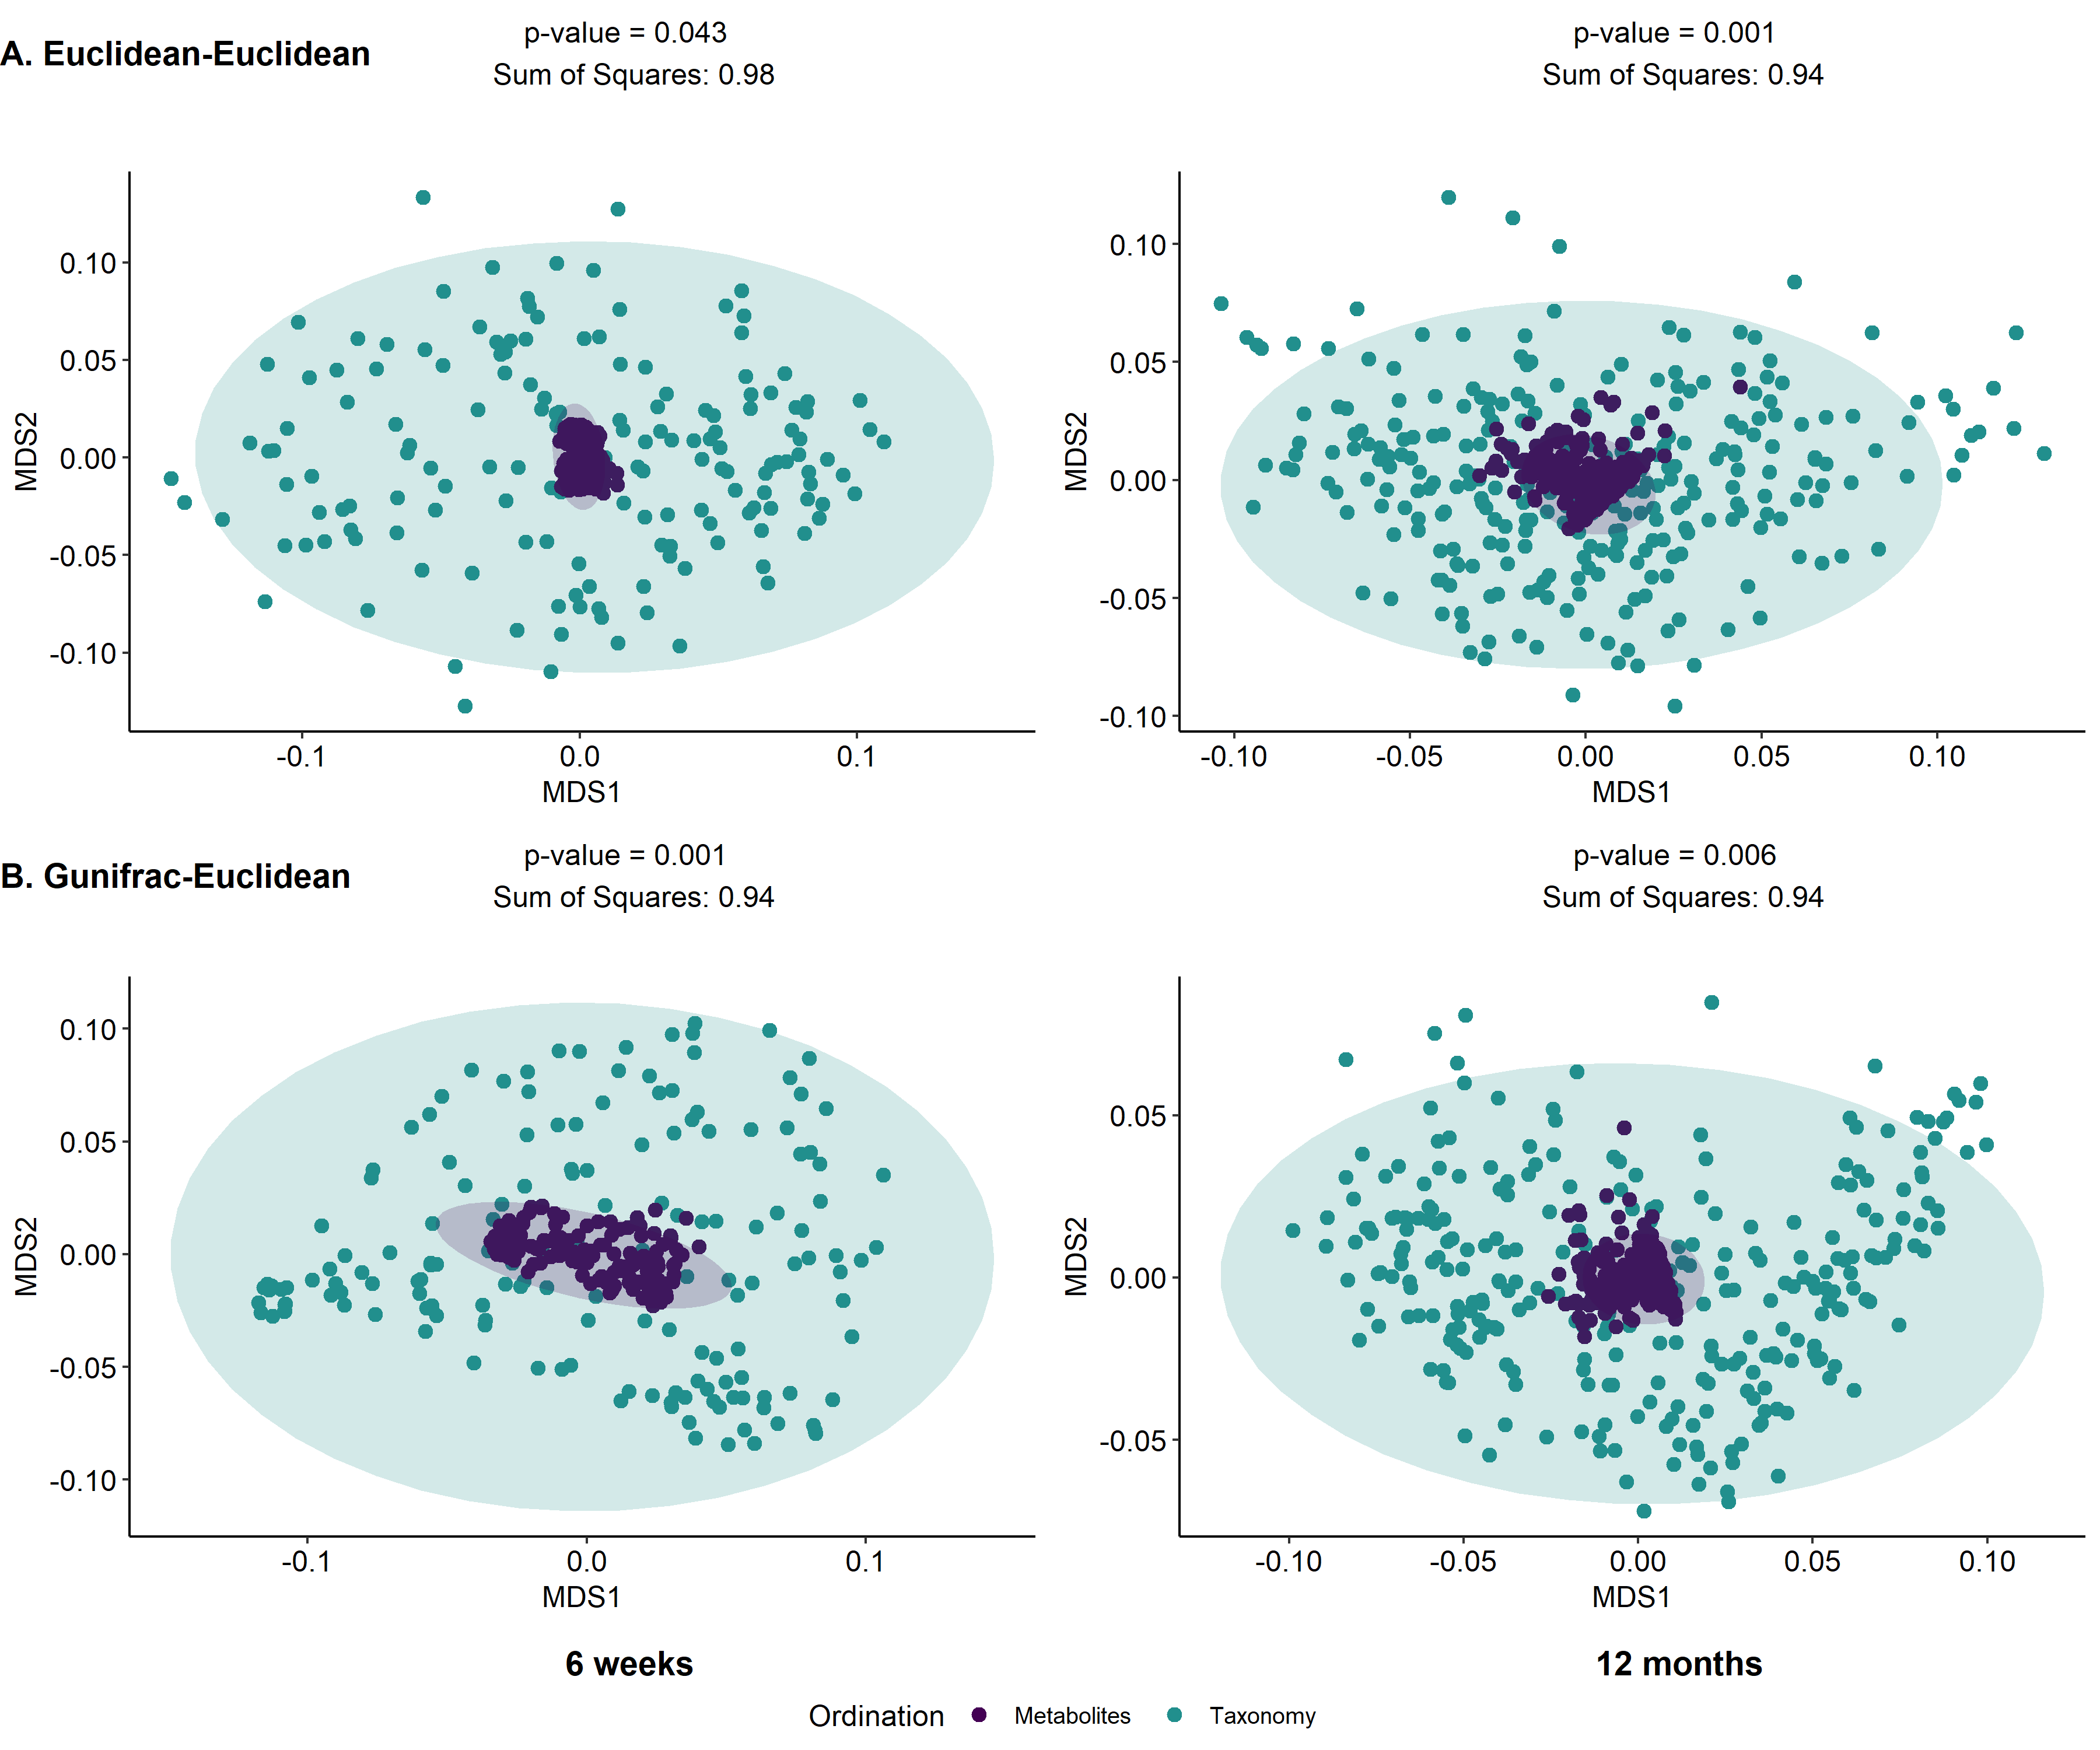
\includegraphics[width=0.95\linewidth]{figures/appB_fs1.png}
    \caption[Inter-omics Procrustes biplots comparing PCoA ordinations of untargeted metabolite profiles and taxonomic relative abundances for 6 weeks (left panels) (n = 158) and 12 months (right panels) (n = 262).]{Inter-omics Procrustes biplots comparing PCoA ordinations of untargeted metabolite profiles and taxonomic relative abundances for 6 weeks (left panels) (n = 158) and 12 months (right panels) (n = 262). Top panels present analyses based on ordinations from Euclidean distances of genus level abundances after centered log ratio transformation and Euclidean distances of arcsine square root transformed metabolite relative abundances. Bottom panel presents analyses based on generalized Unifrac distance of amplicon sequence variant (ASV) relative abundances and Euclidean distances of arcsine square root transformed metabolite relative abundances.}
    \label{fig:b1}
\end{figure}

\begin{figure}[!h]
    \centering
    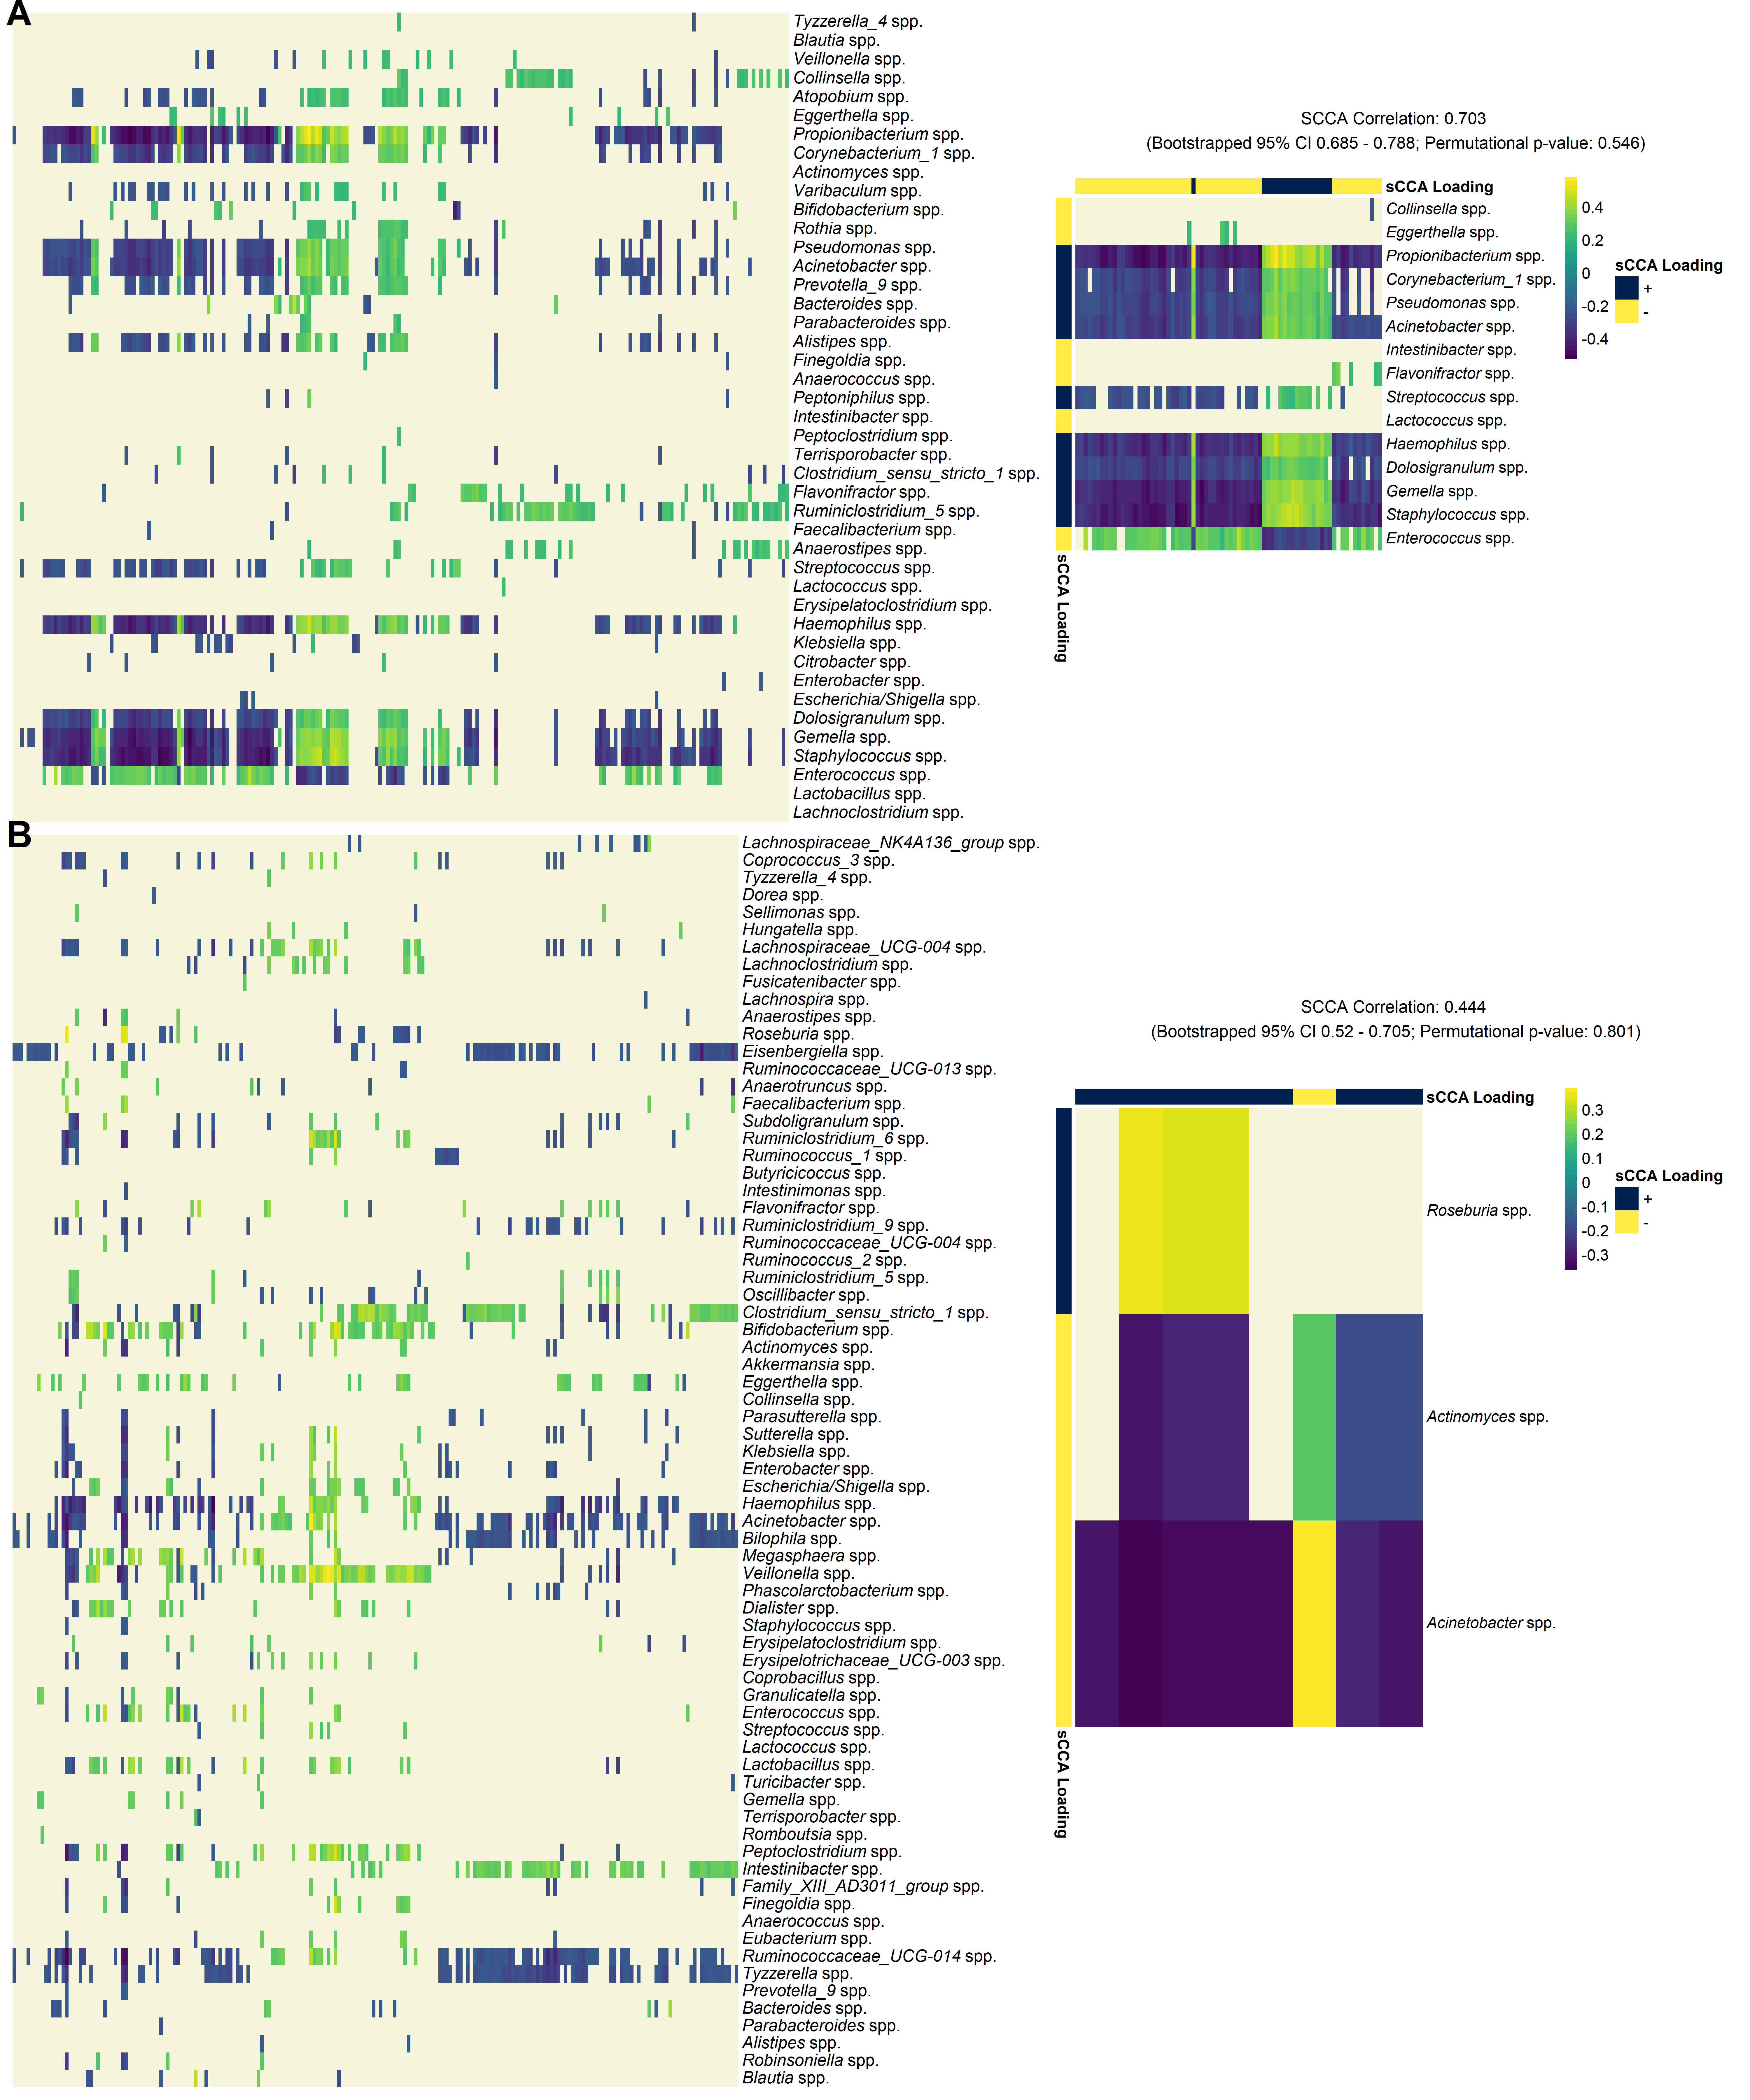
\includegraphics[width=0.95\linewidth]{figures/appB_fs2.png}
    \caption[Pairwise Spearman correlation of metabolite bins and genus-level taxonomic abundances for 6-weeks (panel A, N = 158) and 12-months (panel B, N = 282) infants.]{Pairwise Spearman correlation of metabolite bins and genus-level taxonomic abundances for 6-weeks (panel A, N = 158) and 12-months (panel B, N = 282) infants. Left panel displays the overall correlation pattern, where non-significant correlations are not colored (false discovery rate (FDR) controlled q-value $<$ 0.05). Right panel displays the same heatmap restricted to taxa and metabolites selected by the sparse CCA procedure. Additionally, correlation coefficient of the first sCCA variate pair, bootstrapped 95\% confidence interval and permutation p-value are also reported.}
    \label{fig:b2}
\end{figure}

\begin{figure}[!h]
    \centering
    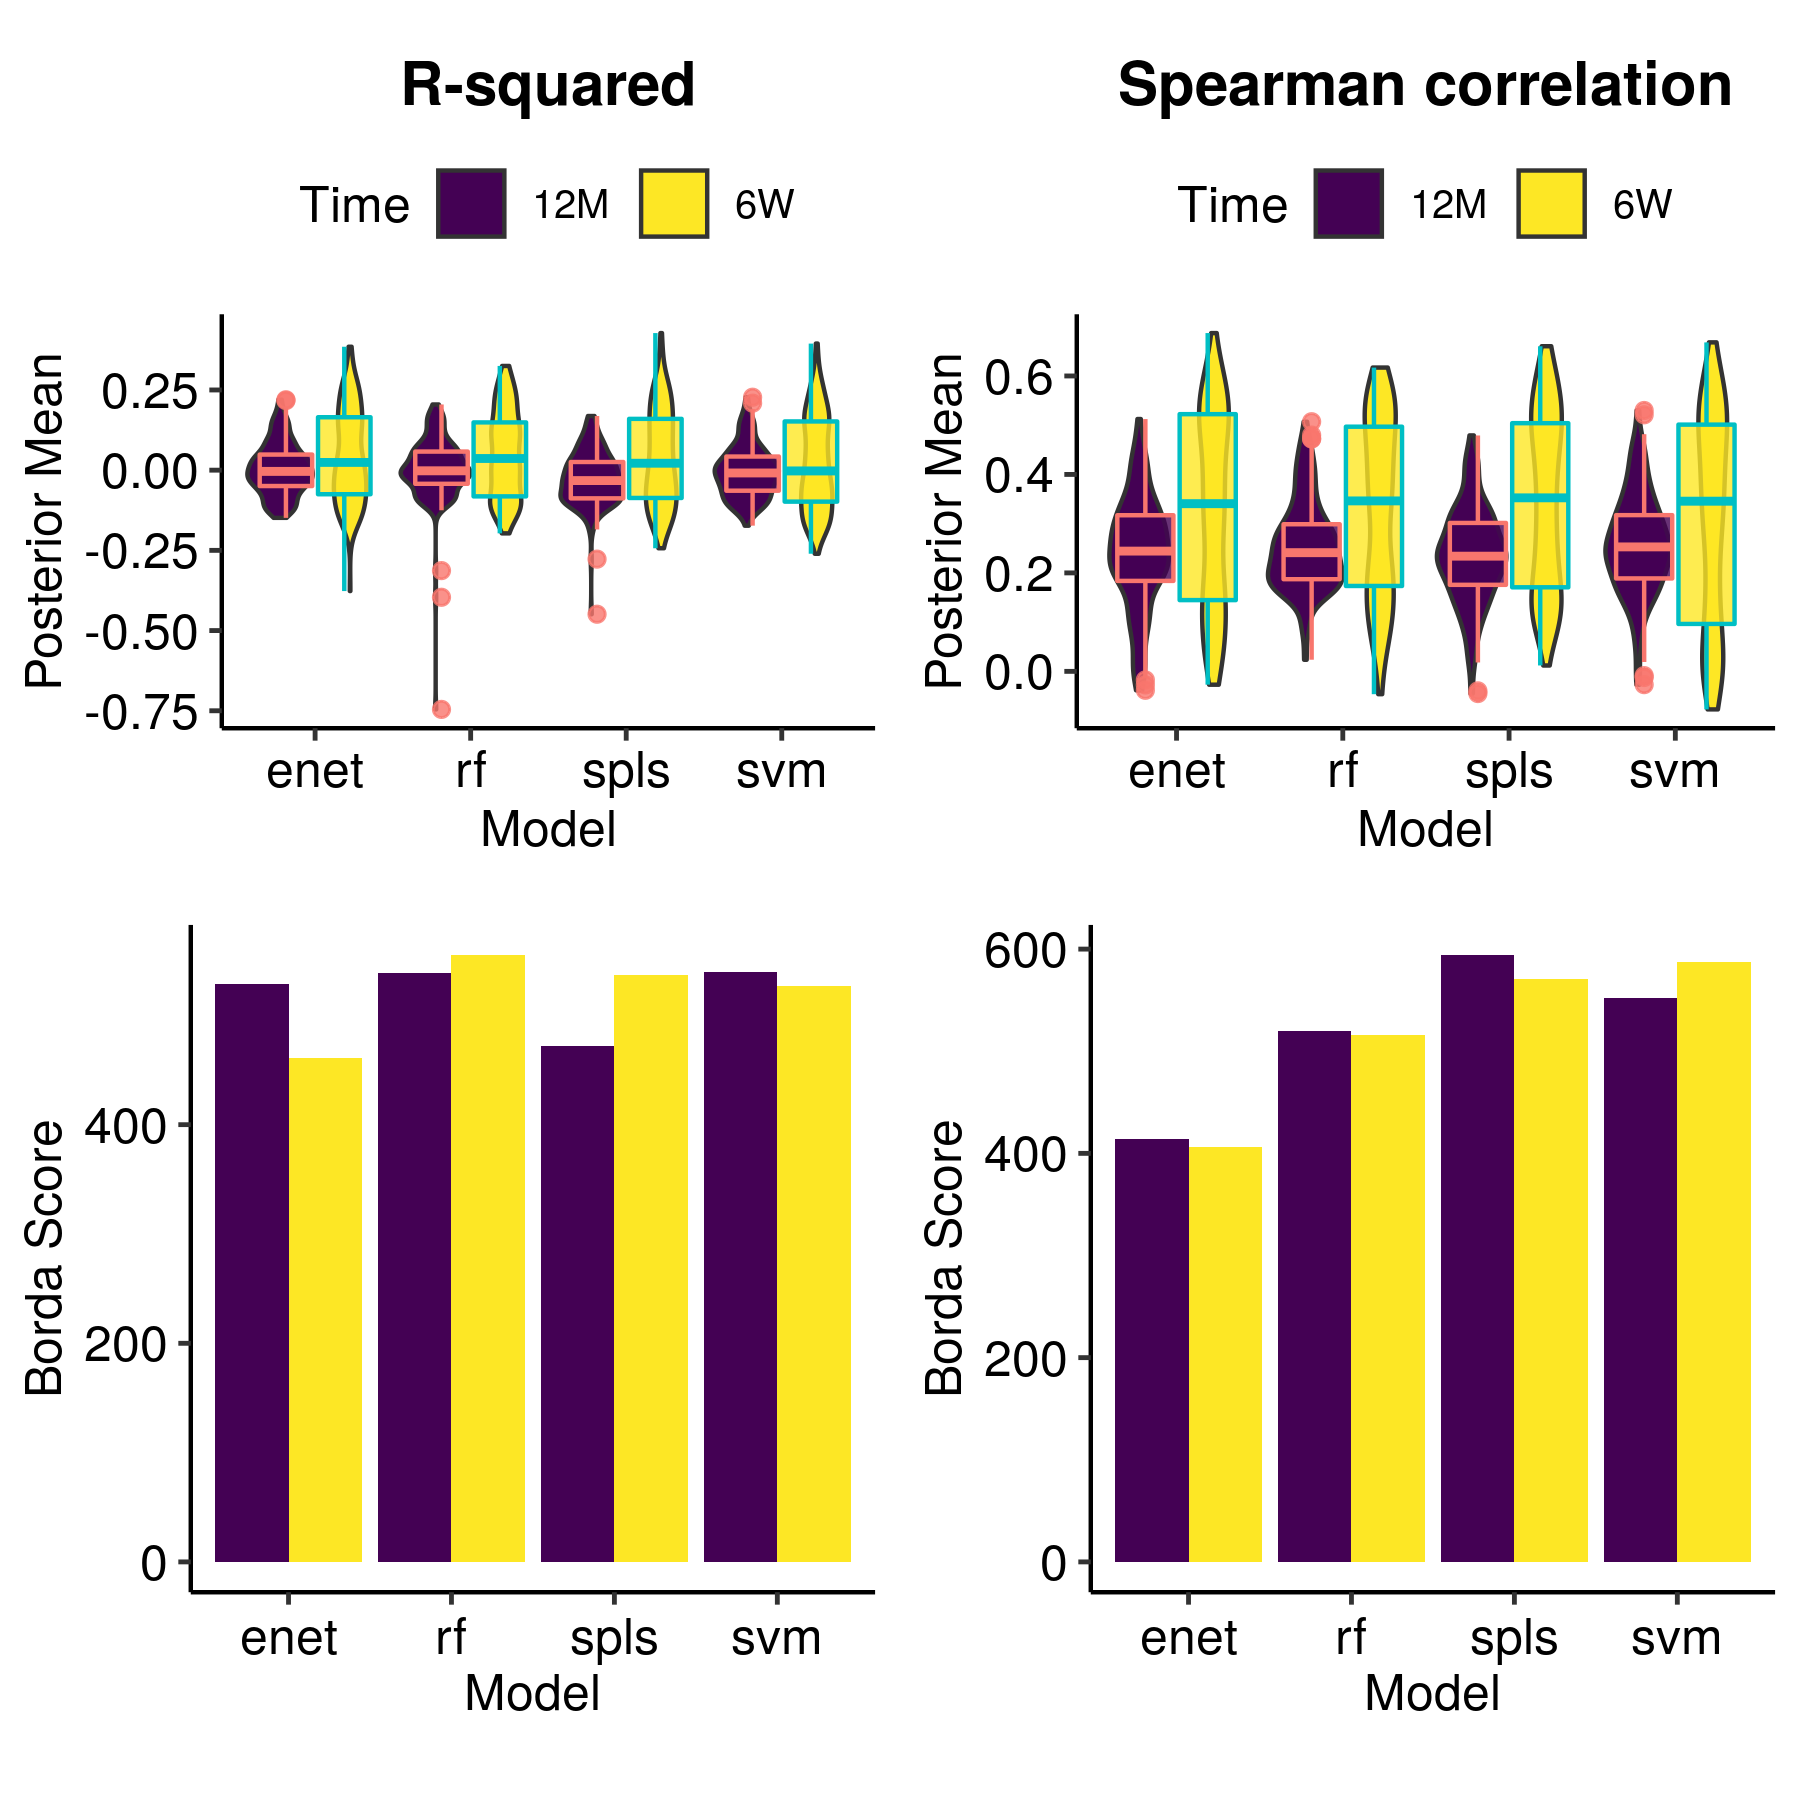
\includegraphics[width=0.95\linewidth]{figures/appB_fs3.png}
    \caption[Comparative analysis predictive model performance across all metabolites in the untargeted dataset for both 6-weeks (n = 158) and 12-months (n = 282) timepoints.]{Comparative analysis predictive model performance across all metabolites in the untargeted dataset for both 6-weeks (n = 158) and 12-months (n = 282) timepoints. Top panel shows superimposed boxplots and violin plots of the distribution of predictive posterior mean for each evaluation metric across all 208 spectral bins. Bottom panels show aggregated model rankings for all metabolites using R-squared (left) and spearman correlation (right) using Borda scores (Methods).}
    \label{fig:b3}
\end{figure}

\begin{figure}[!h]
    \centering
    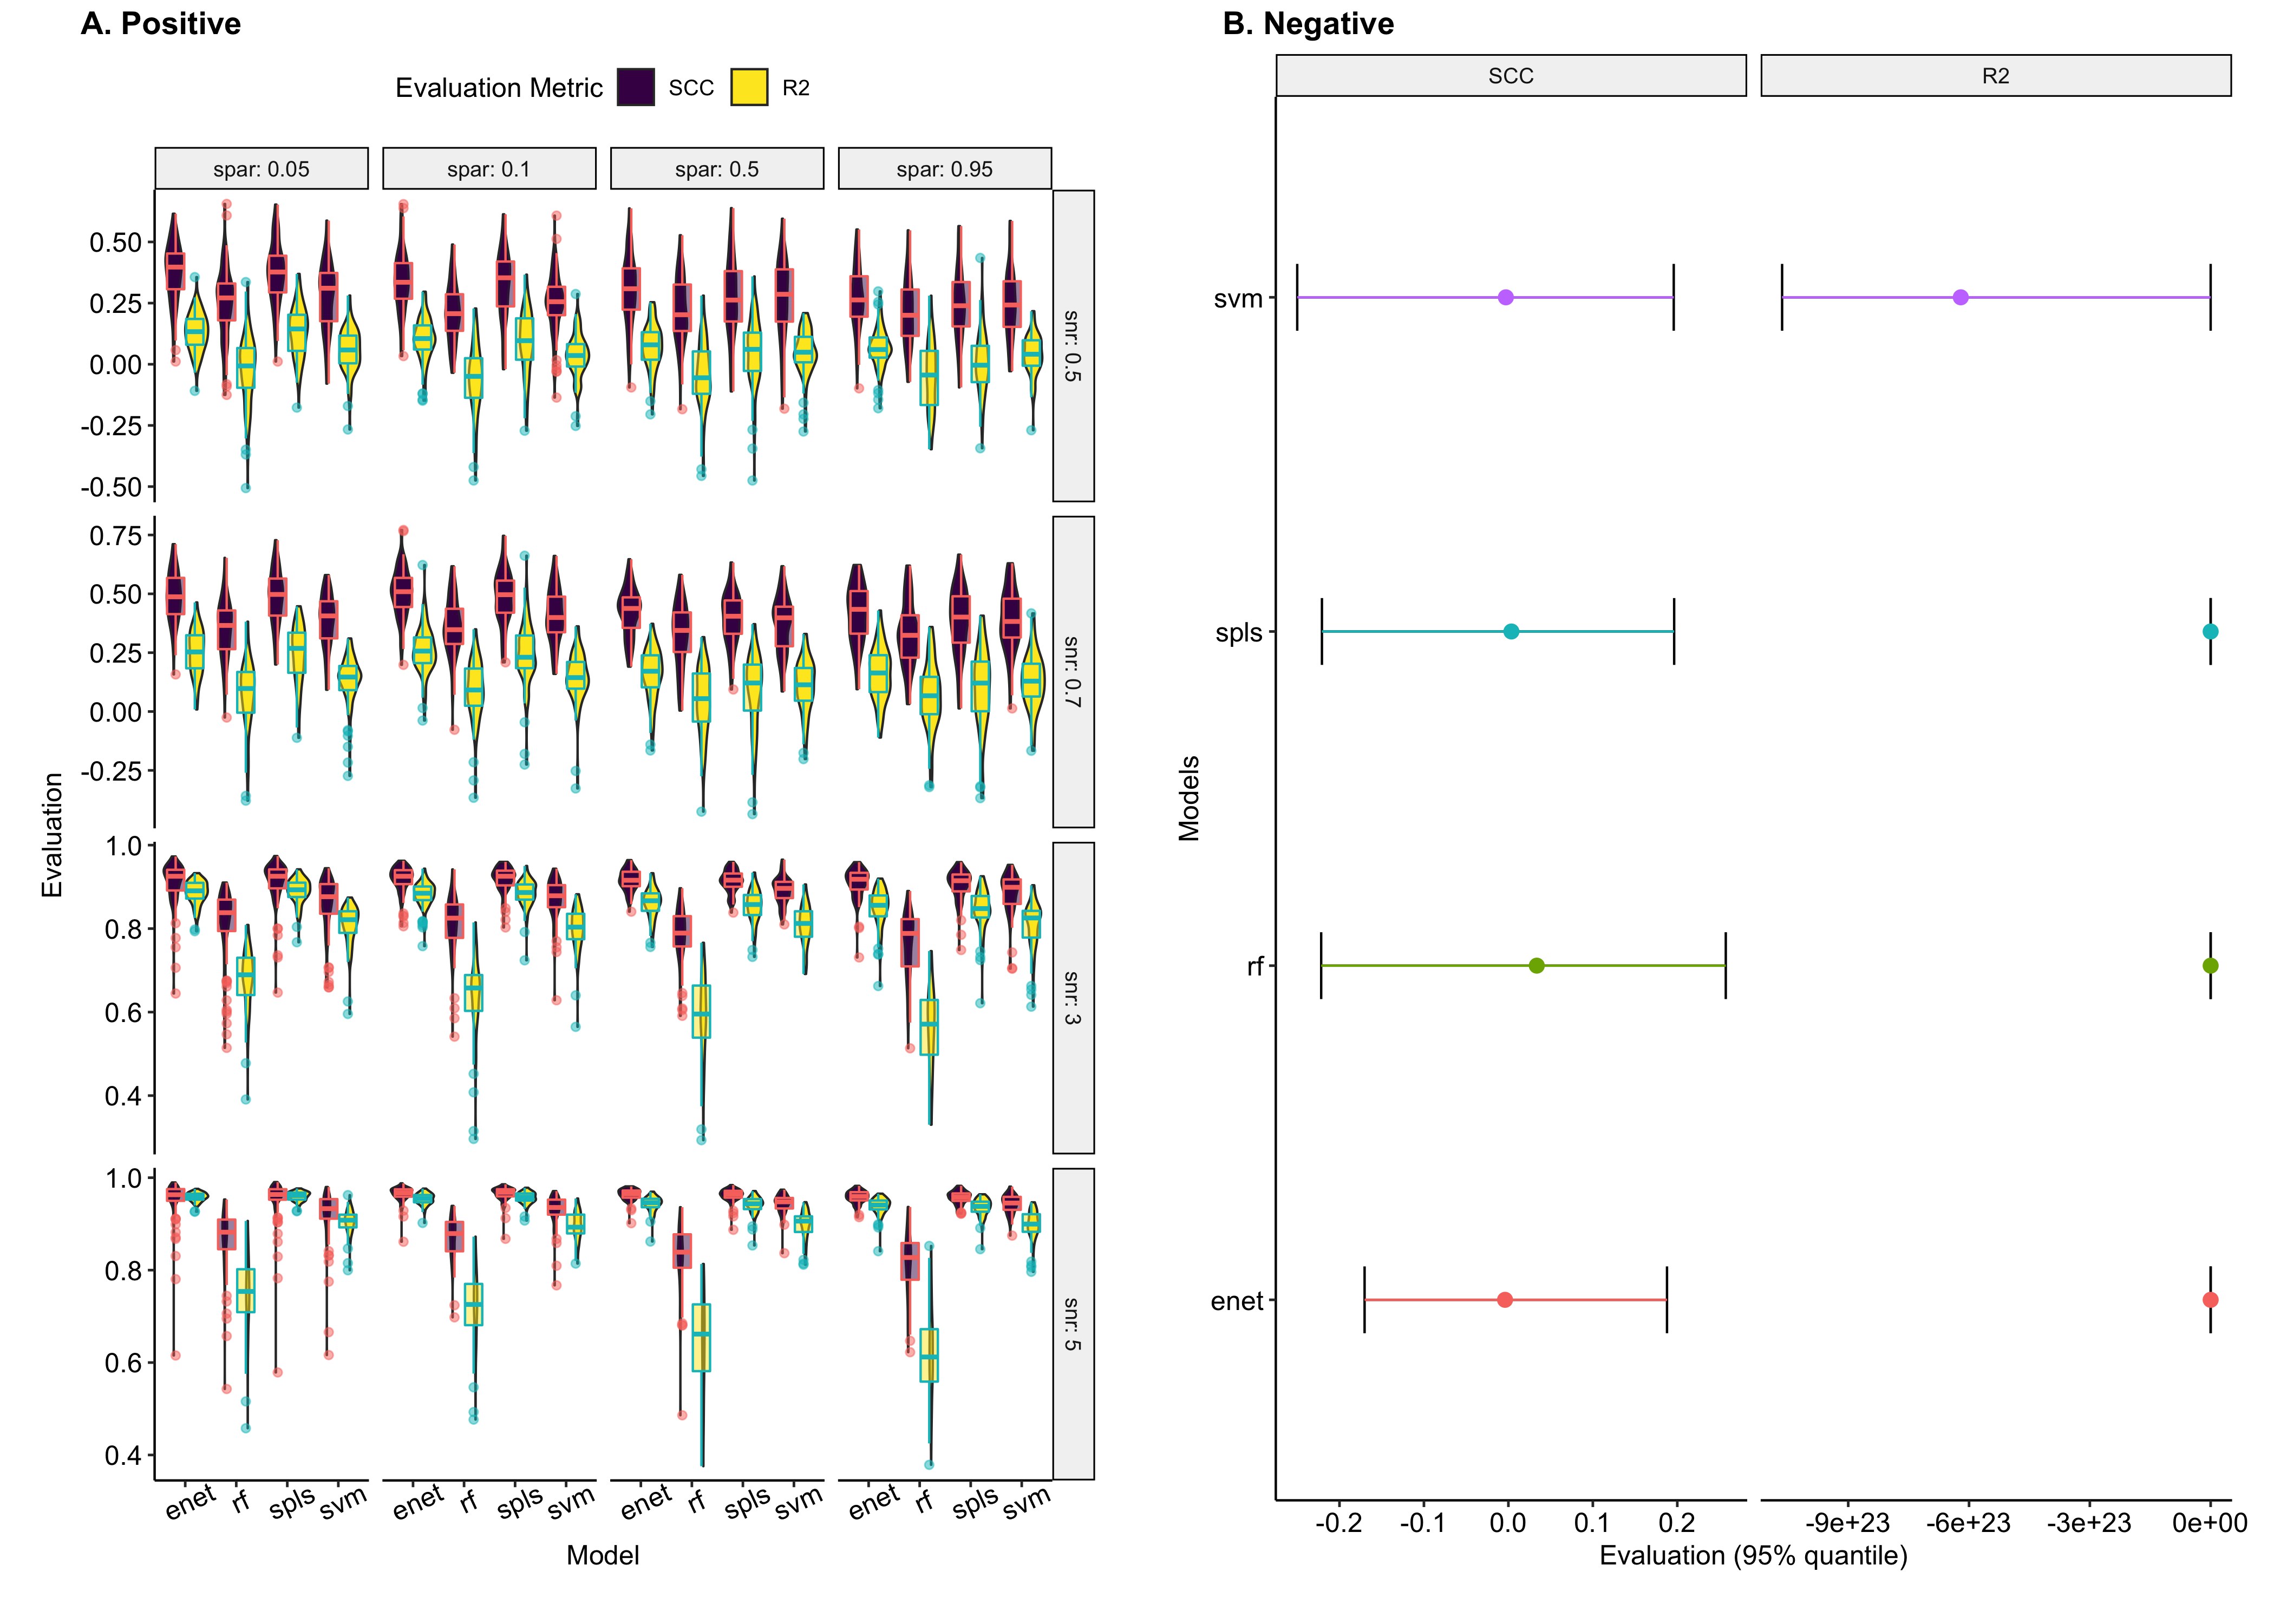
\includegraphics[width=0.95\linewidth]{figures/appB_fs4.png}
    \caption[Results for positive (Panel A) and negative simulations (Panel B)]{Results for positive (Panel A) and negative simulations (Panel B). Positive simulations were conducted based on bootstrapped resamples of the original data (12-month time point) and a normally distributed outcome vector which represented a log-transformed metabolite profile. Different levels of model saturation (horizontal, model sparsity (spar) at 0.05, 0.1, 0.5, 0.95) and effect sizes (vertical, signal-to-noise ratio (snr) at 0.5, 0.7, 3, 5) were assessed, with 100 data sets generated for each setting combination. Negative simulations were conducted based on permutations of the original data (12-month time point), with a total of 1000 permutations. Highly negative outliers were removed for the purposes of visualization.}
    \label{fig:b4}
\end{figure}

\begin{figure}[!h]
    \centering
    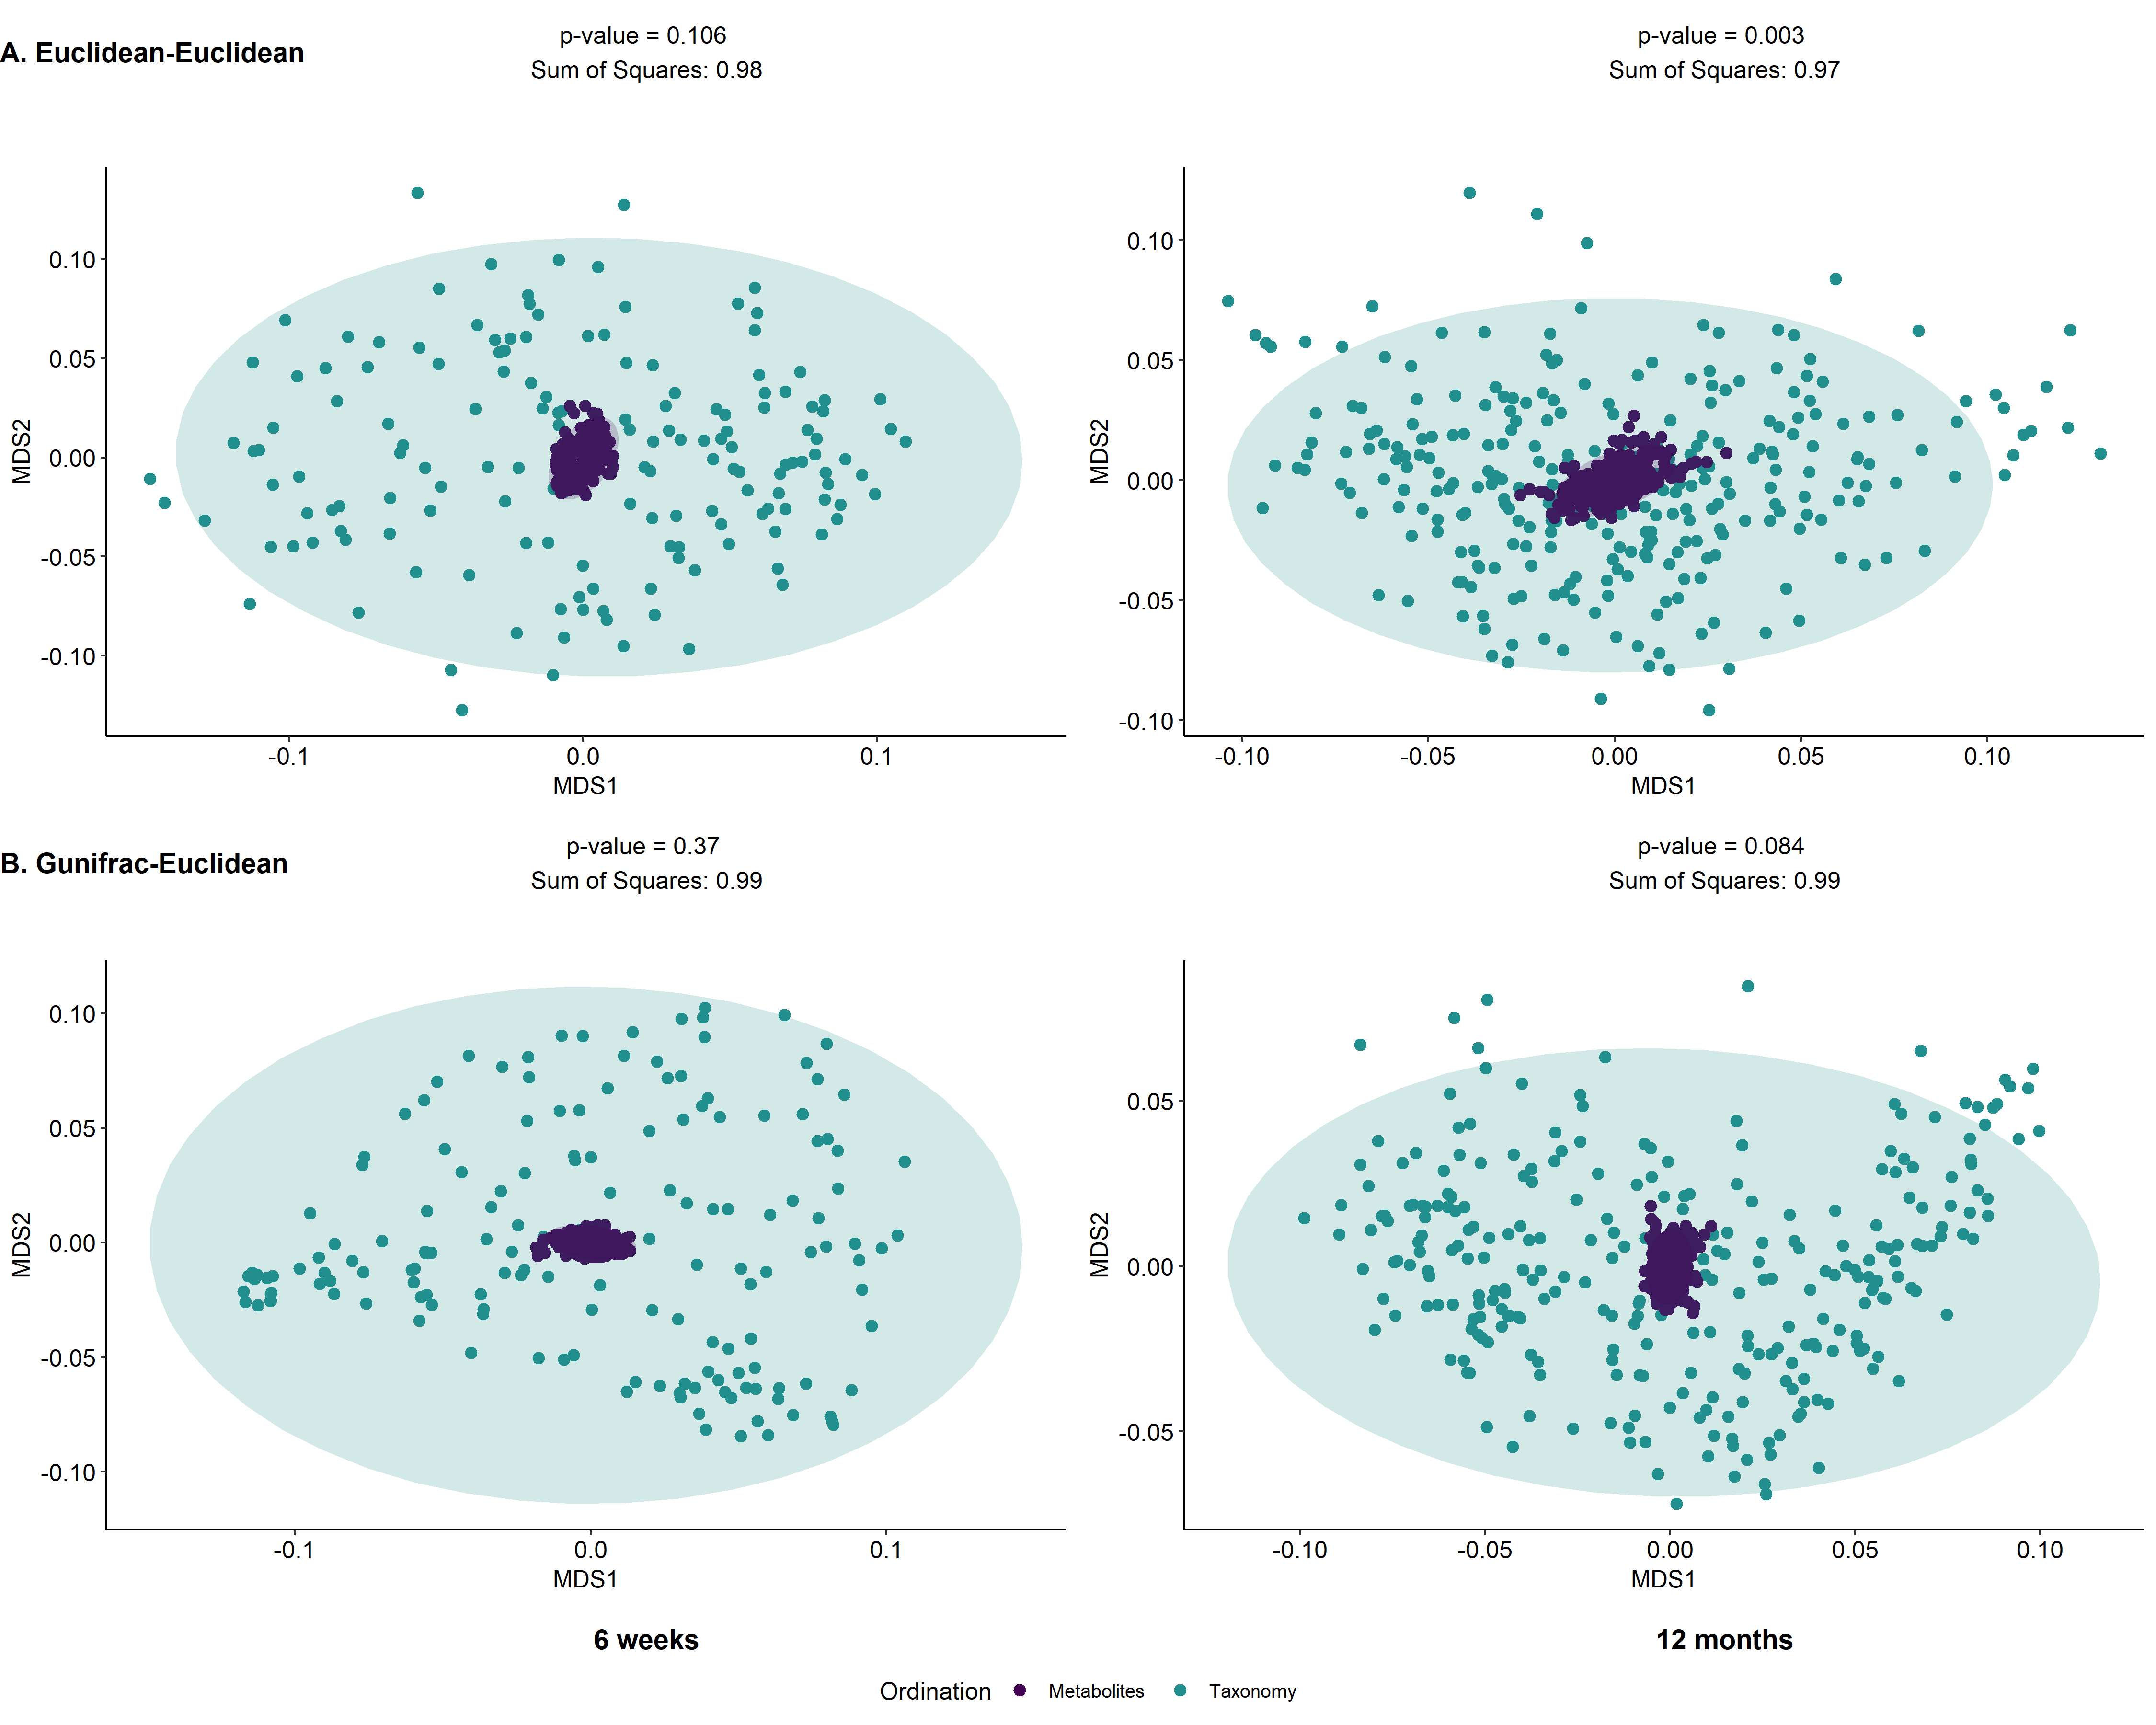
\includegraphics[width=0.95\linewidth]{figures/appB_fs5.png}
    \caption[Inter-omics Procrustes biplots comparing PCoA ordinations of targeted metabolite profiles and taxonomic relative abundances in the sensitivity analyses for 6 weeks (left panels) ($N = 65$) and 12 months (right panels) ($N = 65$)]{Inter-omics Procrustes biplots comparing PCoA ordinations of targeted metabolite profiles and taxonomic relative abundances in the sensitivity analyses for 6 weeks (left panels) ($N = 65$) and 12 months (right panels) ($N = 65$). Top panels present analyses based on ordinations from Euclidean distances of genus level abundances after centered log ratio transformation and Euclidean distances of arcsine square root transformed metabolite relative abundances. Bottom panel presents analyses based on generalized Unifrac distance of amplicon sequence variant (ASV) relative abundances and Euclidean distances of arcsine square root transformed metabolite relative abundances.}
    \label{fig:b5}
\end{figure}

\begin{figure}[!h]
    \centering
    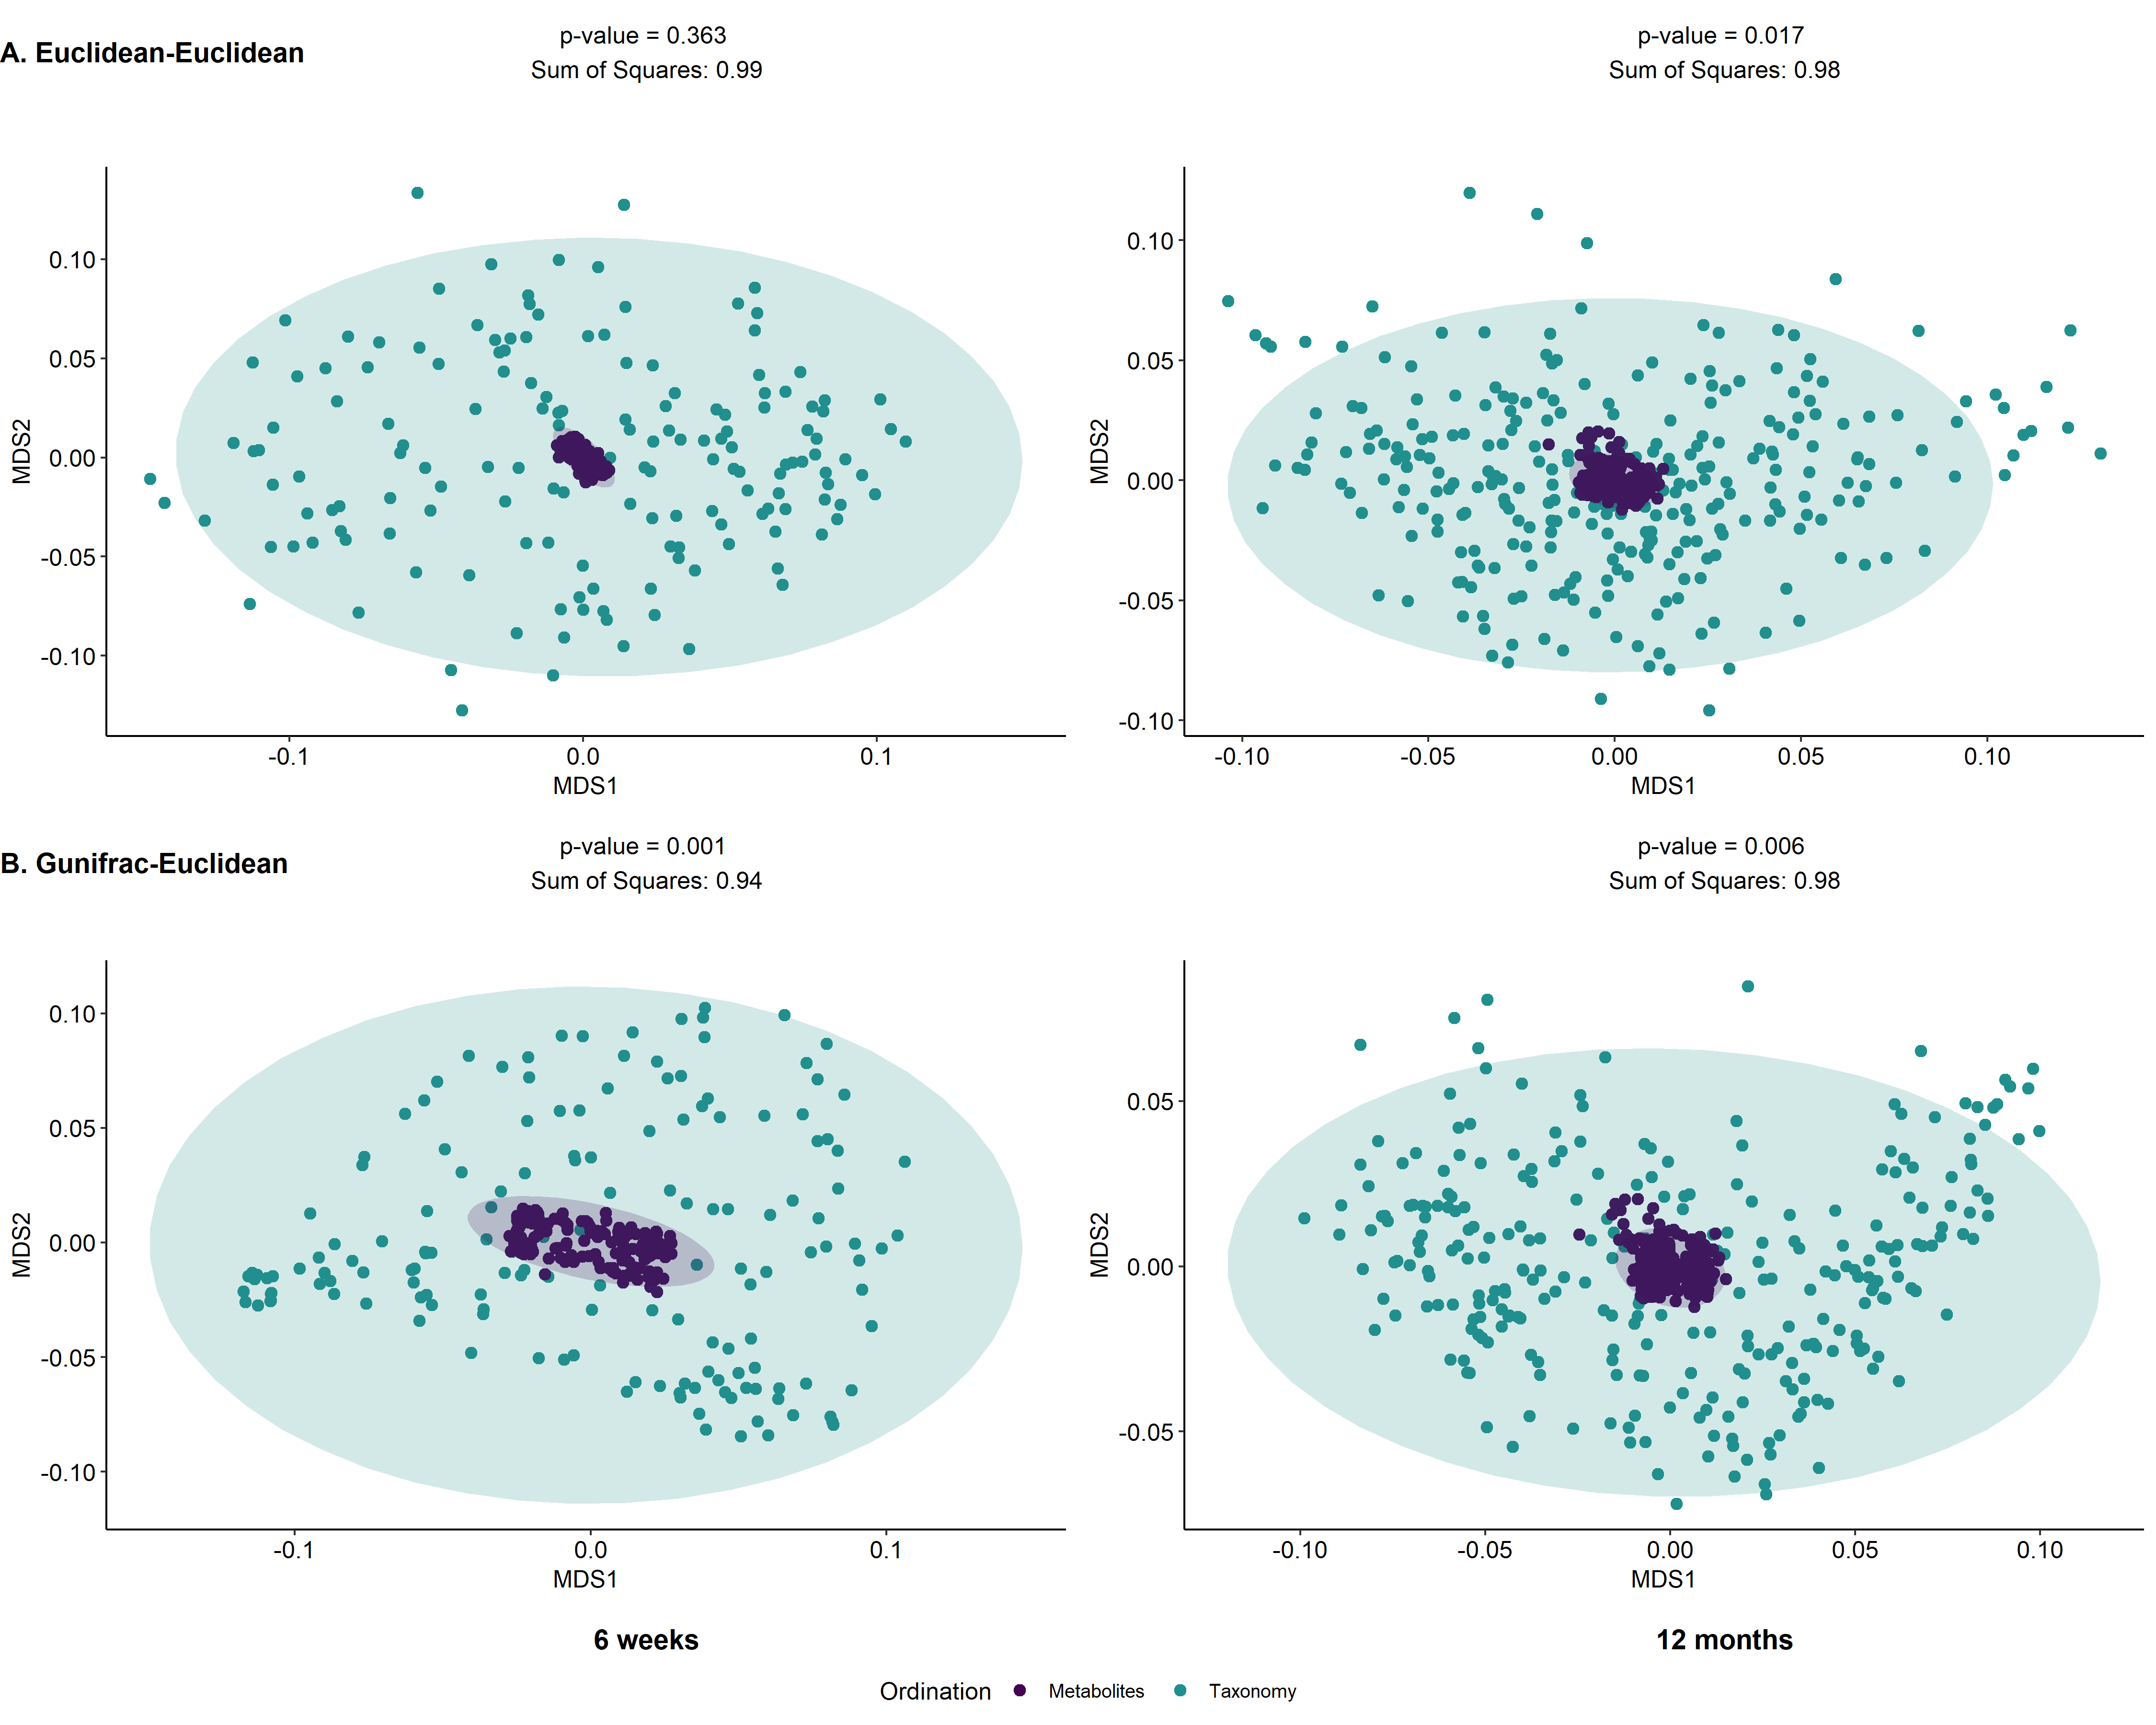
\includegraphics[width=0.95\linewidth]{figures/appB_fs6.png}
    \caption[Inter-omics Procrustes biplots comparing PCoA ordinations of untargeted metabolite bin relative concentrations and taxonomic relative abundances in the sensitivity analyses for 6 weeks (left panels) ($N = 65$) and 12 months (right panels) ($N = 65$)]{Inter-omics Procrustes biplots comparing PCoA ordinations of untargeted metabolite bin relative concentrations and taxonomic relative abundances in the sensitivity analyses for 6 weeks (left panels) ($N = 65$) and 12 months (right panels) ($N = 65$). Top panels present analyses based on ordinations from Euclidean distances of genus level abundances after centered log ratio transformation and Euclidean distances of arcsine square root transformed metabolite relative abundances. Bottom panel presents analyses based on generalized Unifrac distance of amplicon sequence variant (ASV) relative abundances and Euclidean distances of arcsine square root transformed metabolite relative abundances.}
    \label{fig:b6}
\end{figure}

\begin{figure}[!h]
    \centering
    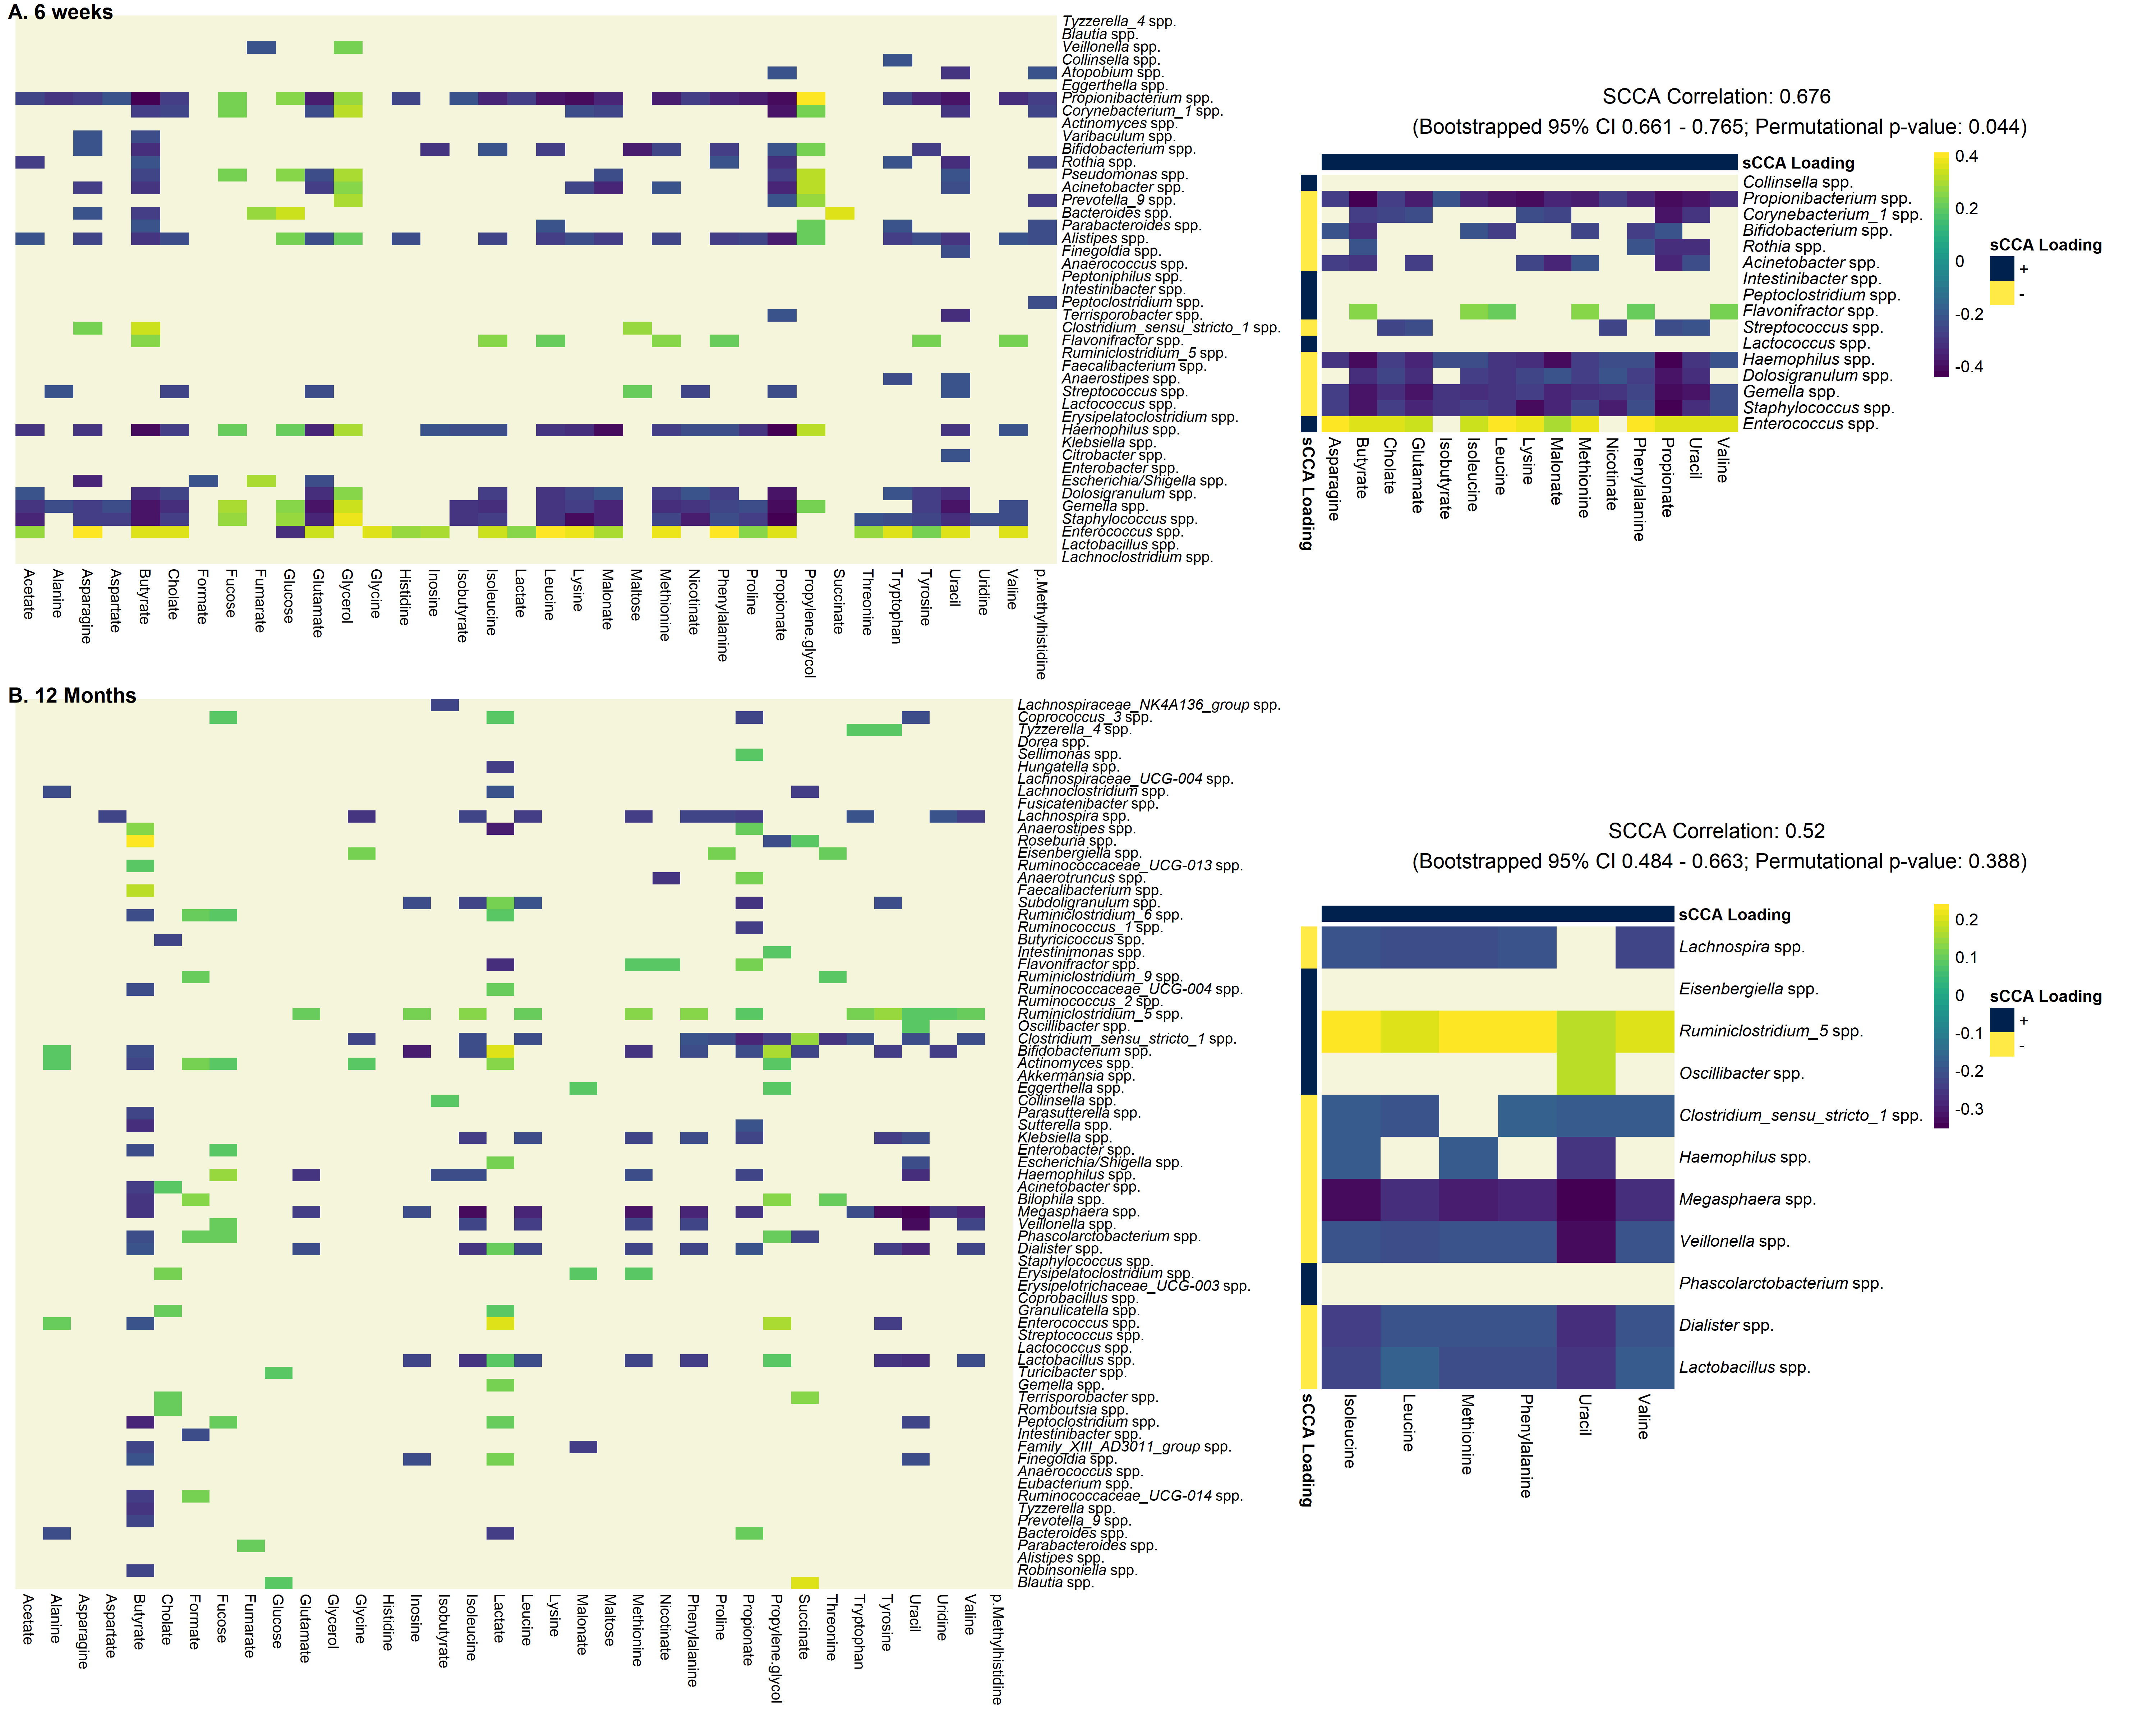
\includegraphics[width=0.95\linewidth]{figures/appB_fs7.png}
    \caption[Pairwise spearman correlation of concentration-fitted targeted metabolite concentrations and genus-level taxonomic abundances for 6-weeks (panel A, $N = 65$) and 12-months (panel B, $N = 65$) infants in sensitivity analyses]{Pairwise spearman correlation of concentration-fitted targeted metabolite concentrations and genus-level taxonomic abundances for 6-weeks (panel A, $N = 65$) and 12-months (panel B, $N = 65$) infants in sensitivity analyses. Left panel displays the overall correlation pattern, where non-significant correlations are not colored (FDR controlled q-value $<$ 0.05). Right panel displays the same heatmap restricted to taxa and metabolites selected by the sCCA procedure. Additionally, correlation coefficient of the first sCCA variate pair, bootstrapped 95\% confidence interval (nboot = 5000) and permutation p-value (nperm = 1000) are also reported.}
    \label{fig:b7}
\end{figure}

\begin{figure}[!h]
    \centering
    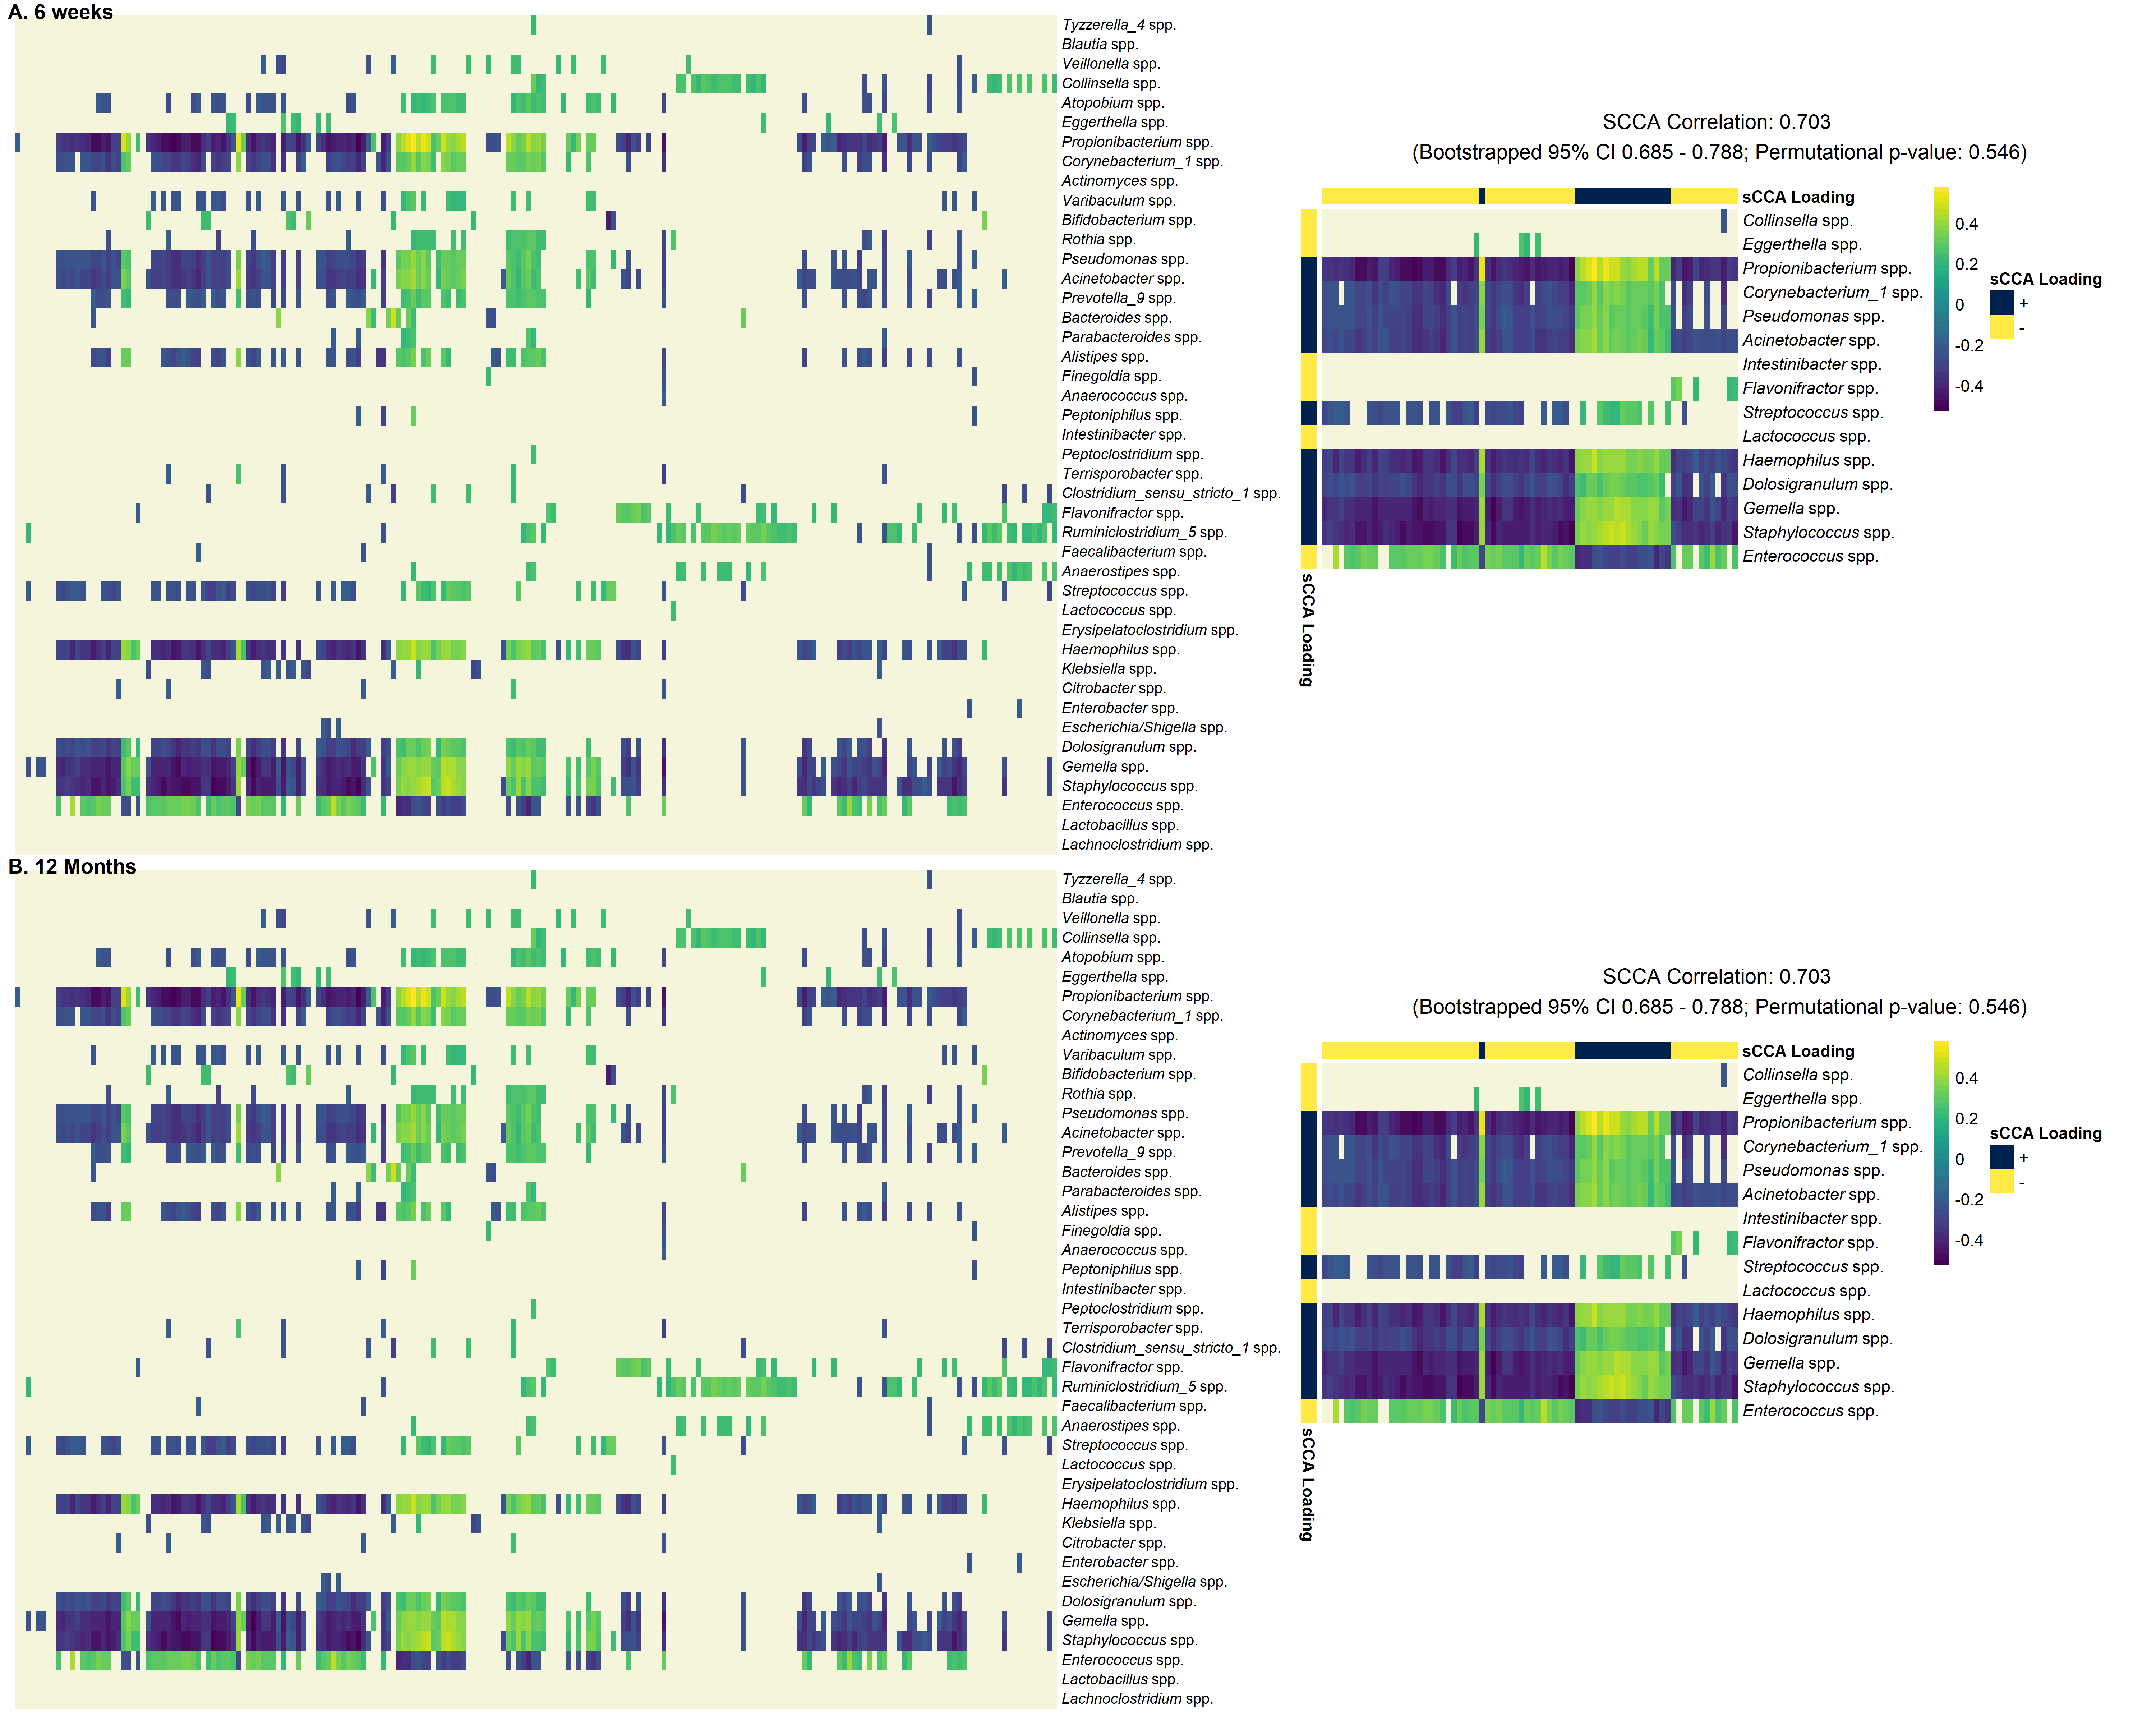
\includegraphics[width=0.95\linewidth]{figures/appB_fs8.png}
    \caption[Pairwise spearman correlation of untargeted metabolite bin relative concentrations and genus-level taxonomic abundances for 6-weeks (panel A, $N = 65$) and 12-months (panel B, $N = 65$) infants in sensitivity analyses]{Pairwise spearman correlation of untargeted metabolite bin relative concentrations and genus-level taxonomic abundances for 6-weeks (panel A, $N = 65$) and 12-months (panel B, $N = 65$) infants in sensitivity analyses. Left panel displays the overall correlation pattern, where non-significant correlations are not colored (FDR controlled q-value $<$ 0.05). Right panel displays the same heatmap restricted to taxa and metabolites selected by the sCCA procedure. Additionally, correlation coefficient of the first sCCA variate pair, bootstrapped 95\% confidence interval (\texttt{nboot} = 5000) and permutation p-value (\texttt{nperm} = 1000) are also reported.}
    \label{fig:b8}
\end{figure}

\begin{figure}[!h]
    \centering
    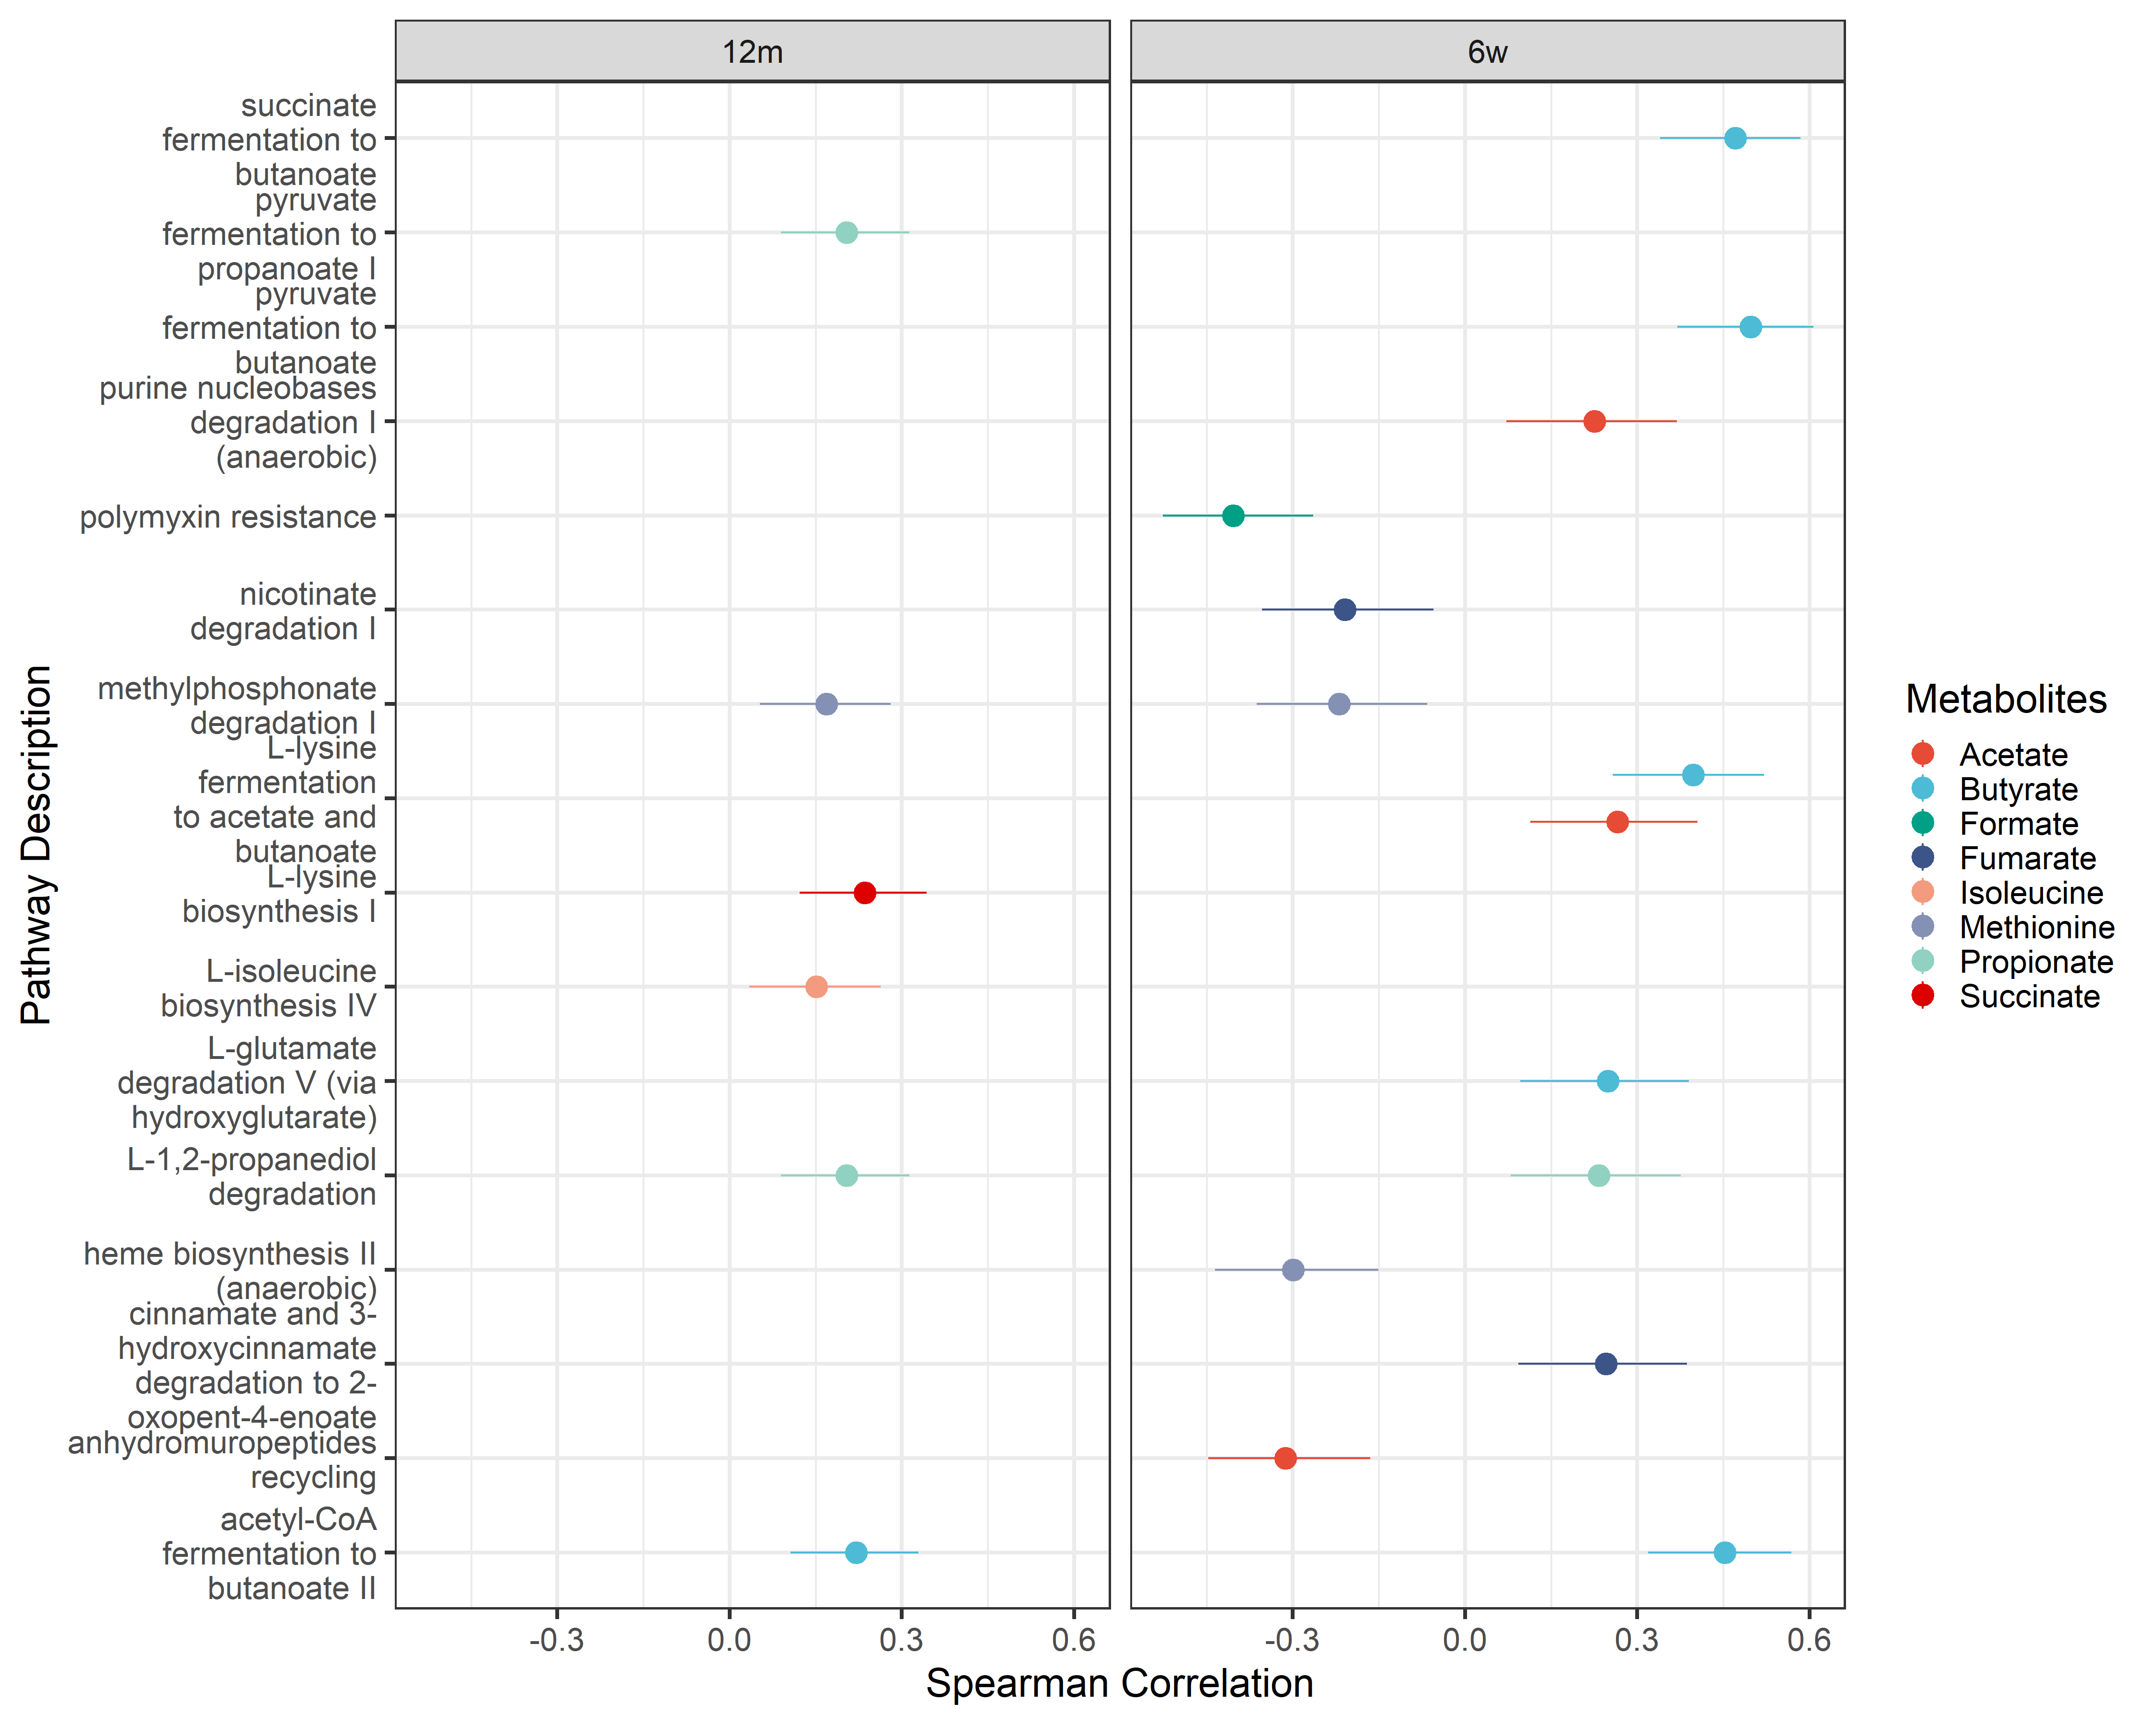
\includegraphics[width=0.95\linewidth]{figures/appB_fs9.png}
    \caption[Spearman correlation coefficients and 95\% confidence intervals of significant correlations (q-value $<$ 0.05) between metabolite concentrations in the targeted data set and the abundances of pathways that produce them]{Spearman correlation coefficients and 95\% confidence intervals of significant correlations (q-value $>$ 0.05) between metabolite concentrations in the targeted data set and the abundances of pathways that produce them. Pathway abundances were obtained via PICRUSt2 predictions, with pathway-metabolite relationship retrieved from MetaCyc database. Both 6-week ($N = 158$) and 12-month ($N = 282$) samples are represented.}
    \label{fig:b9}
\end{figure}

\begin{figure}[!h]
    \centering
    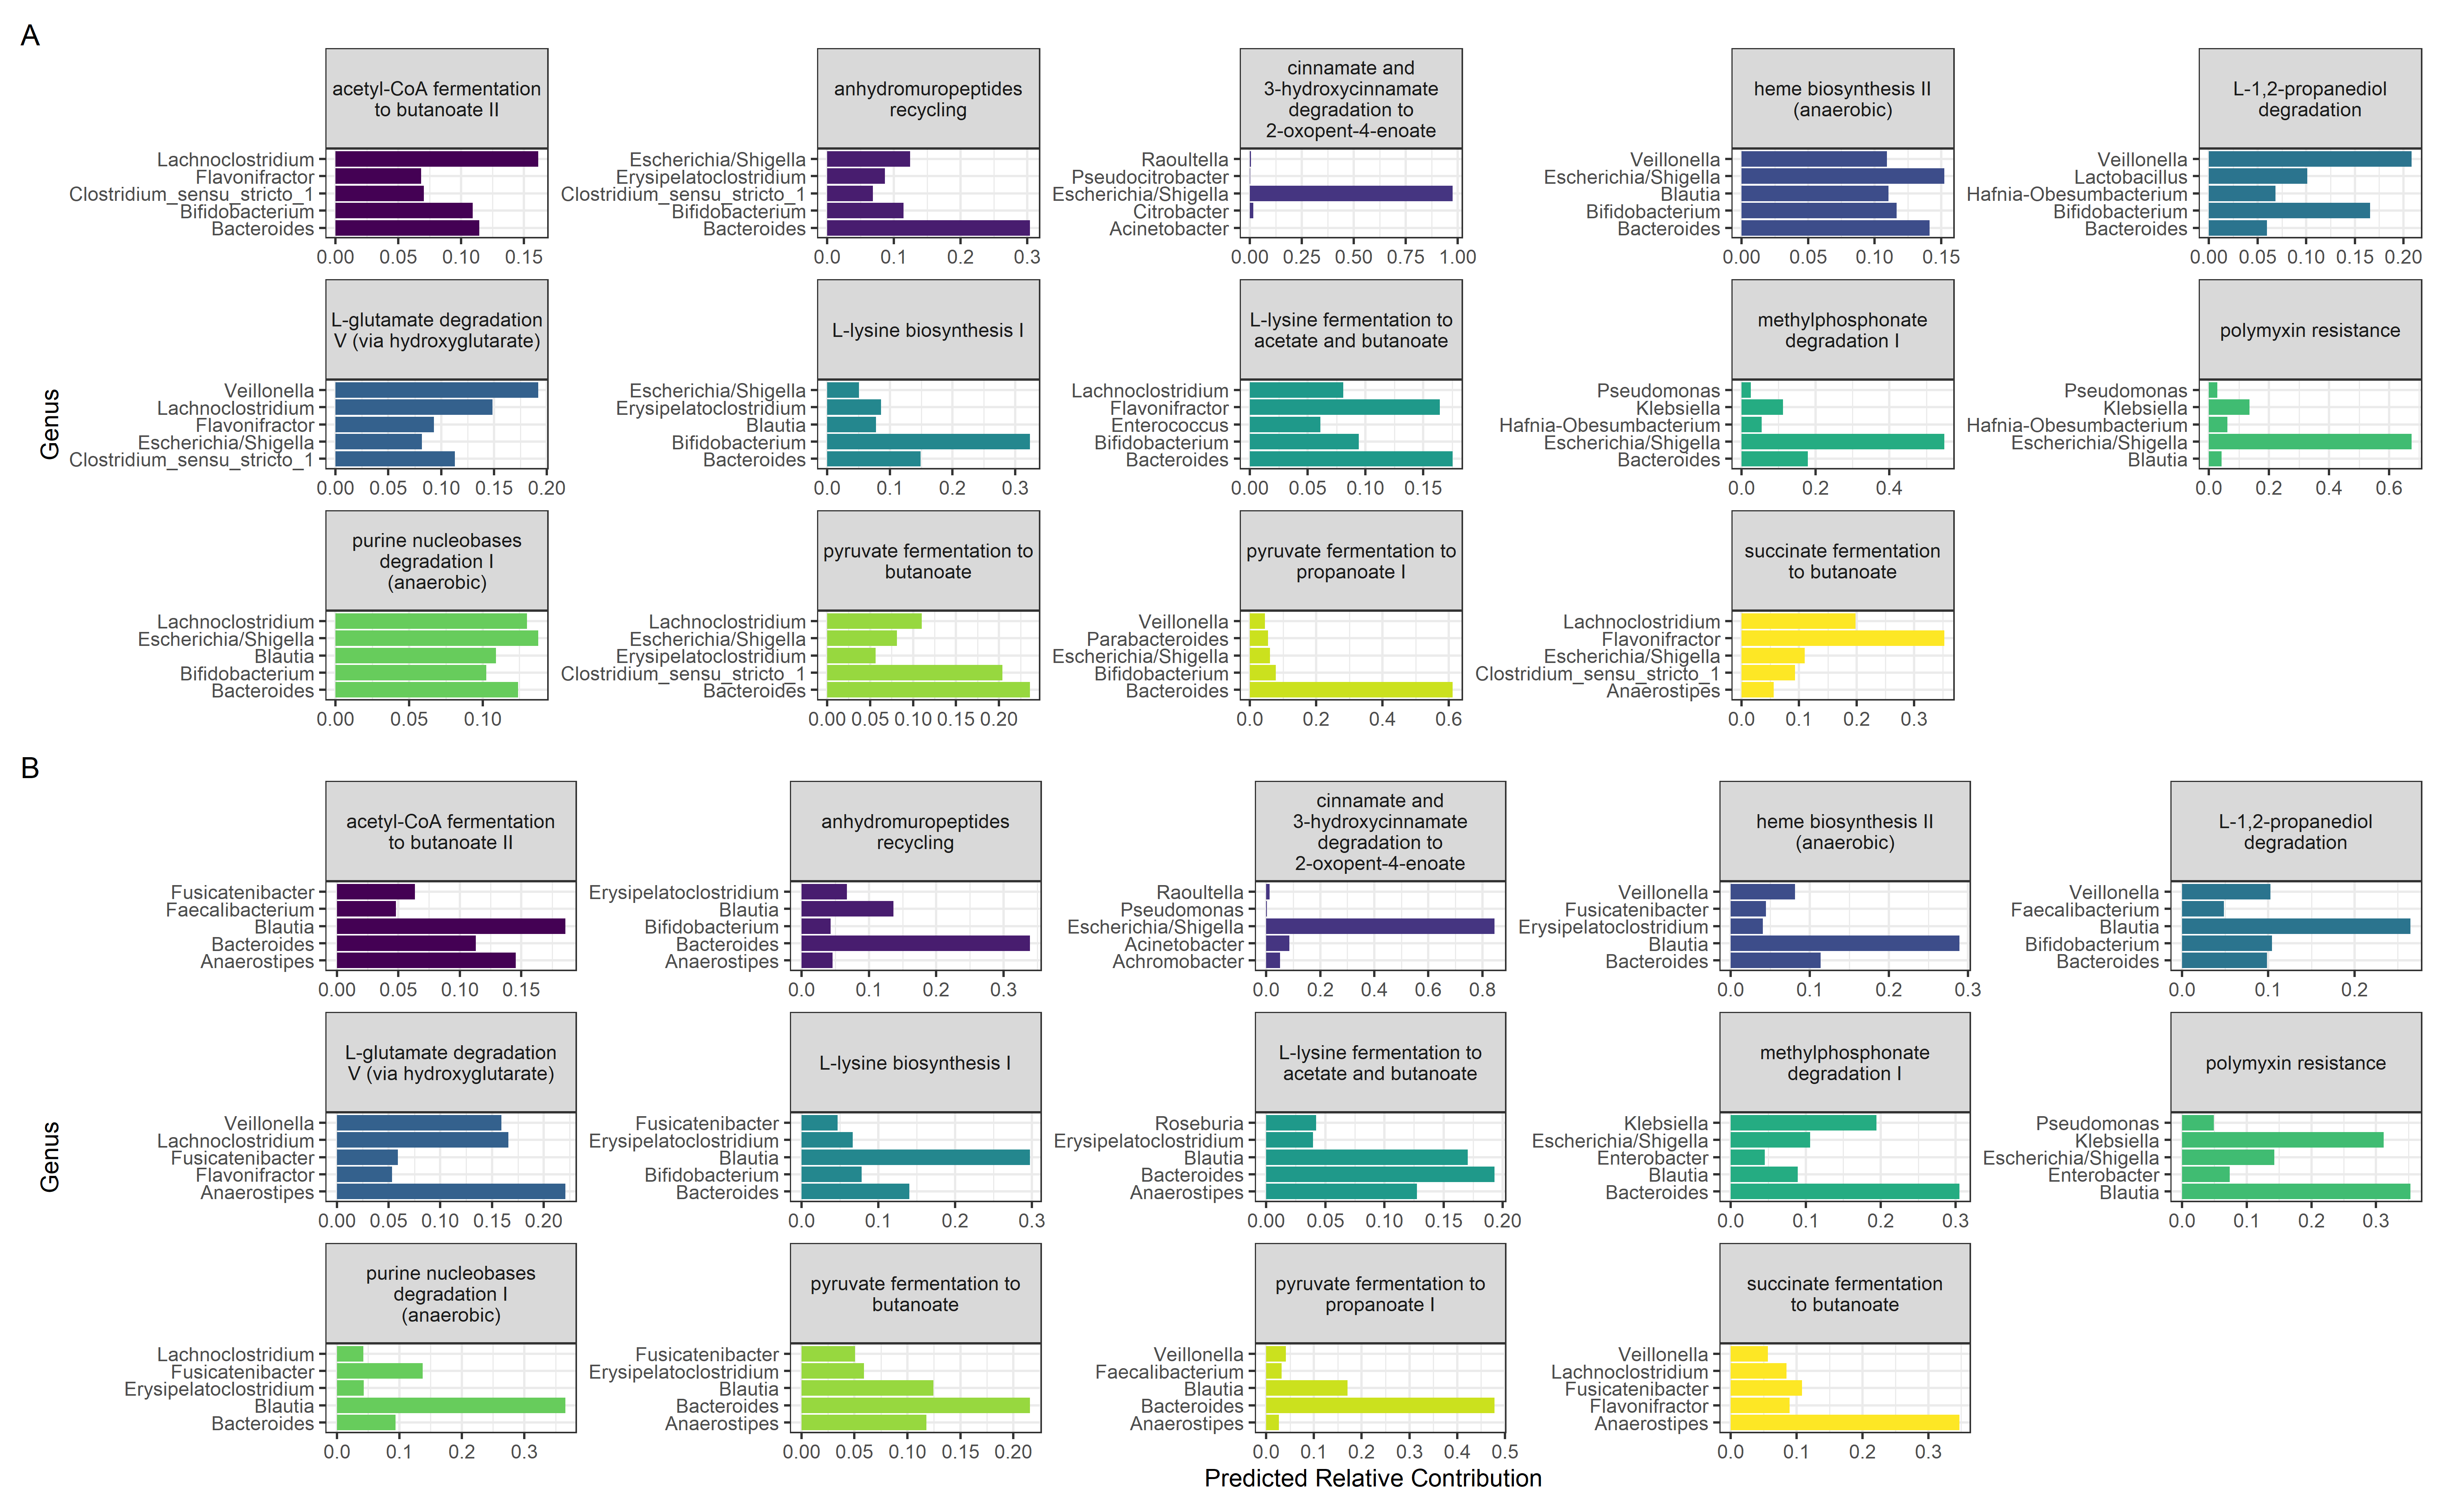
\includegraphics[width=0.95\linewidth]{figures/appB_fs10.png}
    \caption[Top five contributors at the Genus level for each significantly correlated pathway-metabolite pair obtained using observed metabolite concentrations and predicted pathway abundances (Spearman correlation with q-value $<$ 0.05)]{Top five contributors at the Genus level for each significantly correlated pathway-metabolite pair obtained using observed metabolite concentrations and predicted pathway abundances (Spearman correlation with q-value < 0.05). Panel A represents 6-week samples while panel B represents samples at 12-months. Relative contributions are calculated as the total number of copies of genes mapped to a pathway across all samples per Genus over the total number of gene copies assigned to that pathway.}
    \label{fig:b10}
\end{figure}

\begin{figure}[!h]
    \centering
    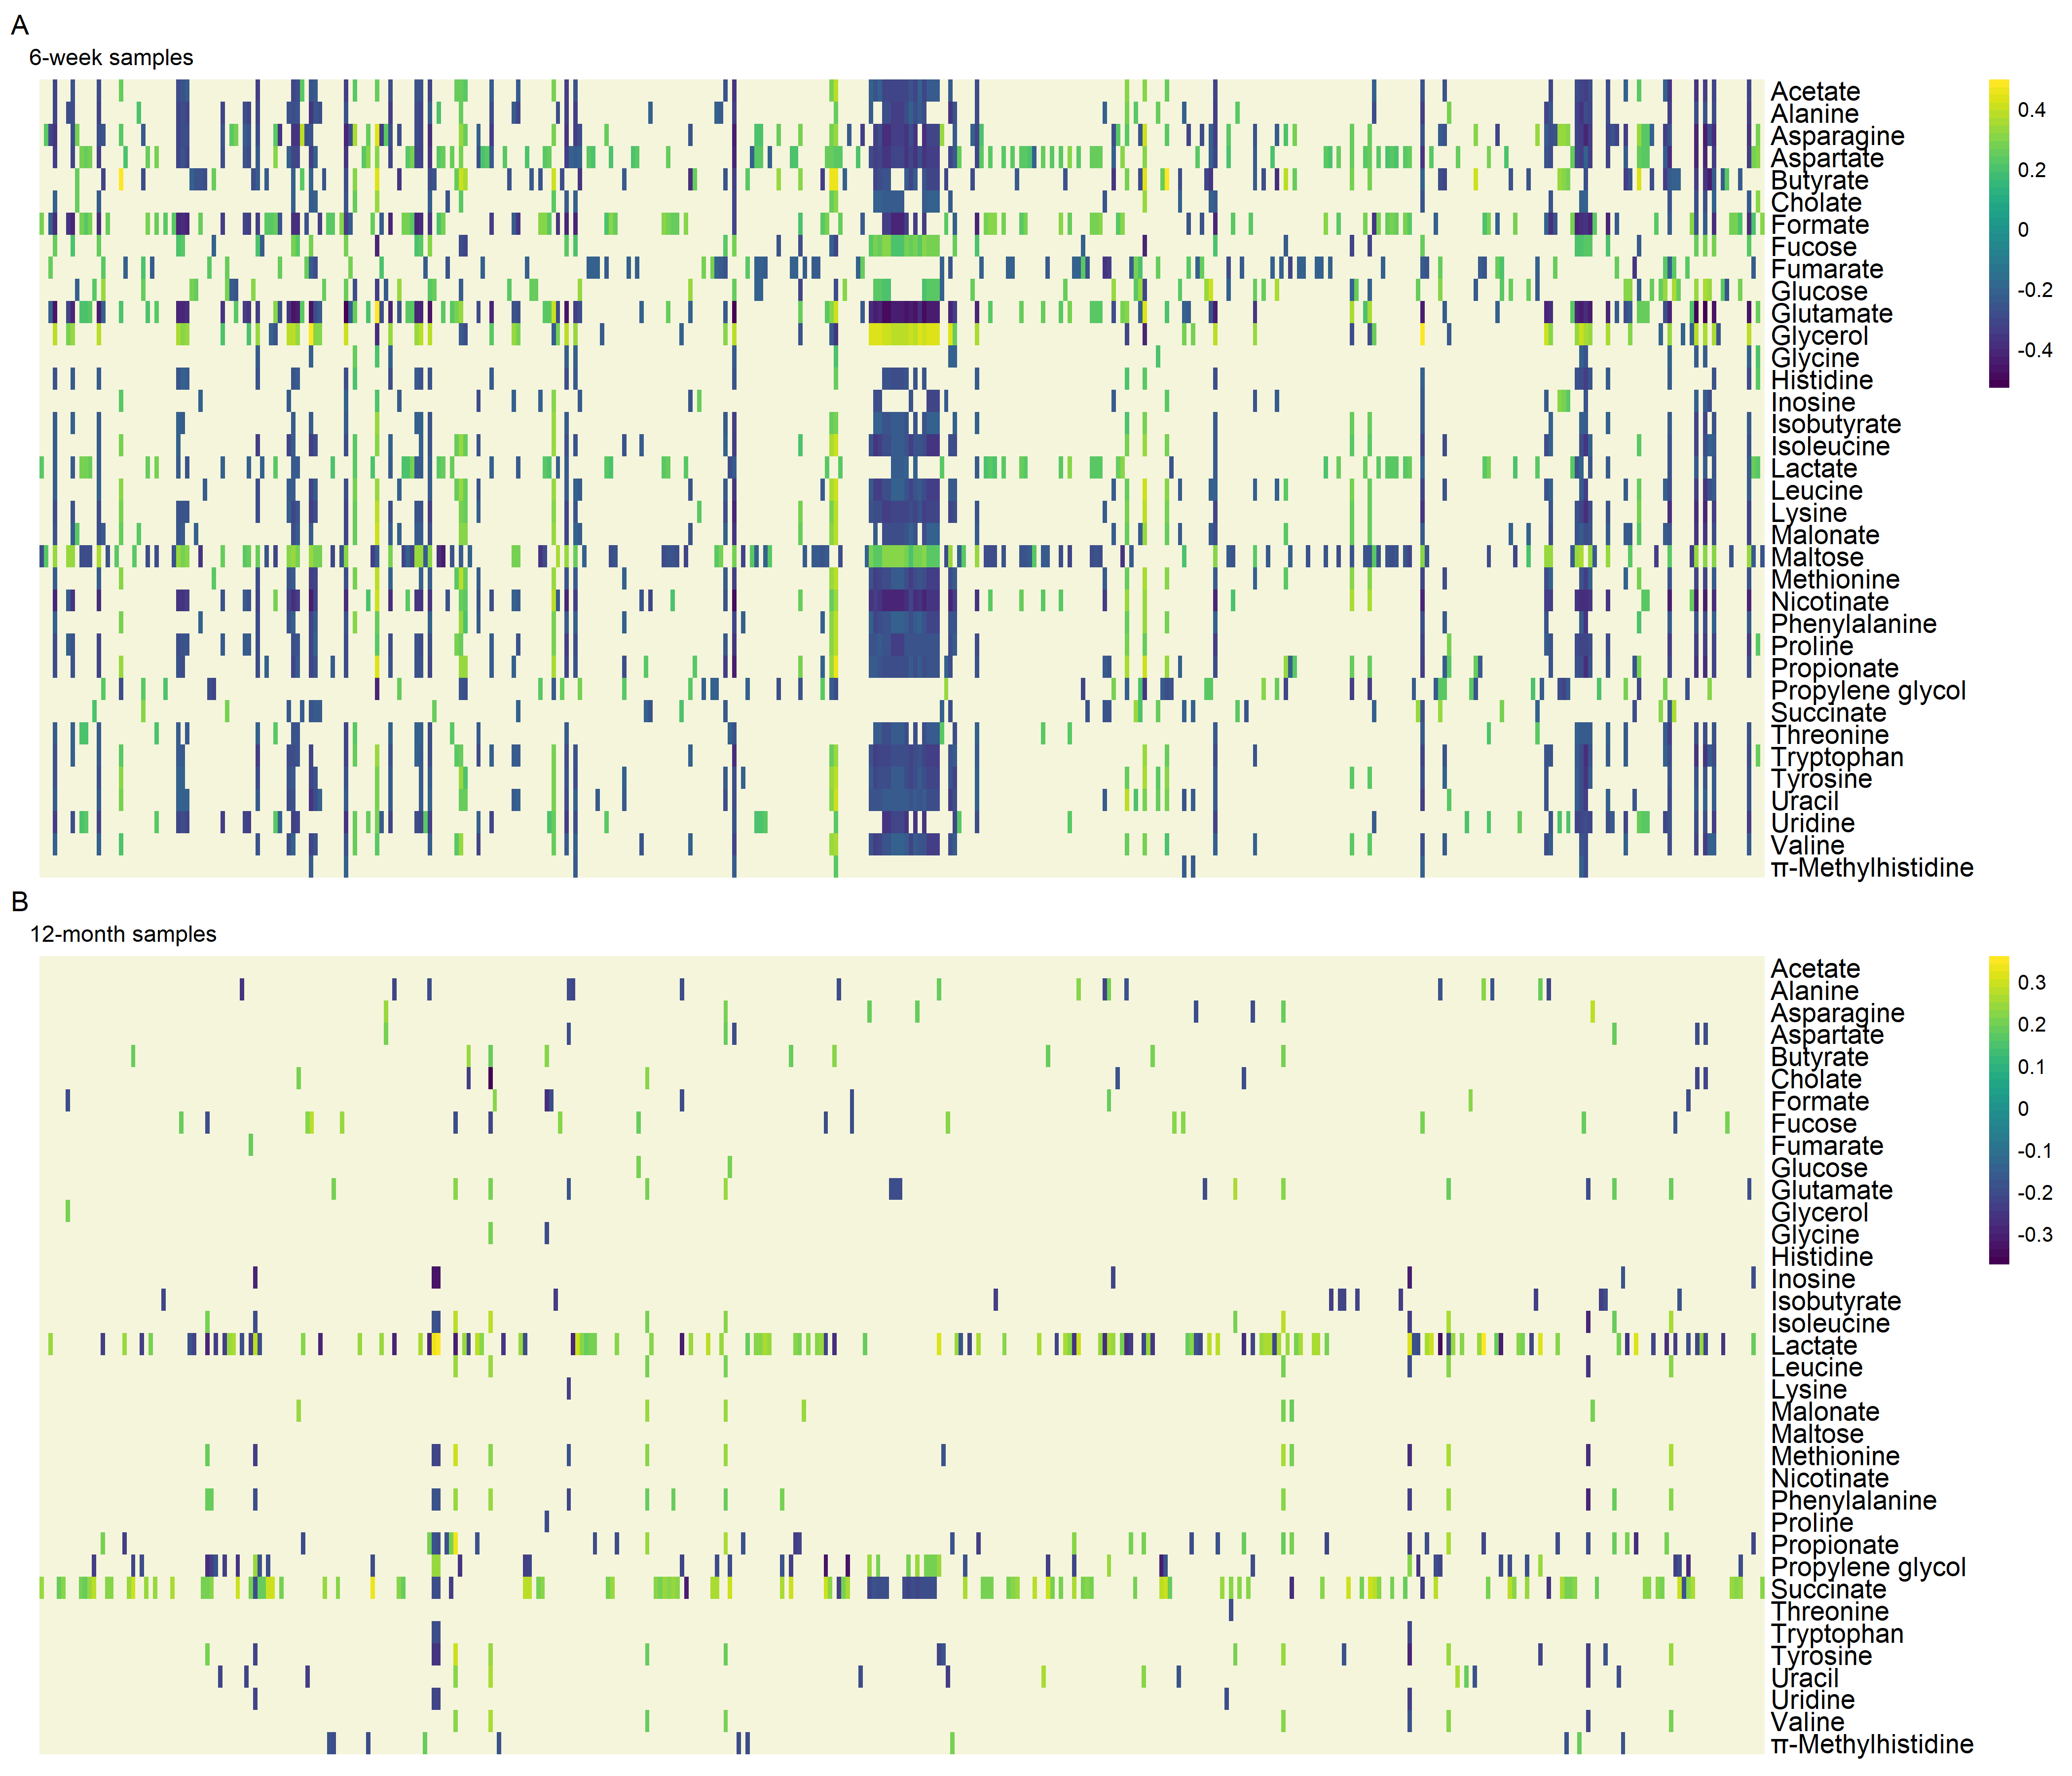
\includegraphics[width=0.95\linewidth]{figures/appB_fs11.png}
    \caption[Heatmap representing overall spearman correlations between predicted pathway abundances (obtained via PICRUSt2) and metabolite concentrations in the targeted data set regardless of pathway-metabolite annotations]{Heatmap representing overall spearman correlations between predicted pathway abundances (obtained via PICRUSt2) and metabolite concentrations in the targeted data set regardless of pathway-metabolite annotations. Both 6-week ($N = 158$) (Panel A) and 12-month ($N = 282$) (Panel B) samples are presented. Non-significant correlations (q-value $>$ 0.05) are not colored.}
    \label{fig:b11}
\end{figure}





 
 
